% Preamble
\documentclass[11pt, proquest] {uwthesis} [2017/04/14]

\usepackage{color}
\usepackage{xspace}
\usepackage{graphicx}
\usepackage{siunitx}
\usepackage{amsmath}
\usepackage{enumitem}

\DeclareMathOperator*{\argmin}{argmin}
\DeclareSIUnit\gauss{G}

\begin{document}

% Functions
\newcommand{\todo}[1]{\textbf{\color{red}{TODO: #1}}}
\newcommand{\note}[1]{\textbf{\color{blue}{NOTE: #1}}}

% Lengths
\newdimen\fdh
\fdh=8em % Height of a single Feynman Diagram

% General aliases
\newcommand{\tsm}{the Standard Model\xspace}
\newcommand{\smpp}{the Standard Model of Particle Physics\xspace}
\newcommand{\uw}{the University of Washington\xspace}

\newcommand{\alphaQED}{\alpha_{_{QED}}}

% g-2 aliases
\newcommand{\gmtwo}{$g\hbox{--}2$\xspace}
\newcommand{\mugmtwo}{$(g\hbox{--}2)_\mu$\xspace}
\newcommand{\wa}{$\omega_a$\xspace}

\newcommand{\fps}{fixed probe system\xspace}

\newcommand{\bmagic}{\SI{1.4513}{\tesla}\xspace}
\newcommand{\rmagic}{\SI{7.112}{\meter}\xspace}
\newcommand{\pmagic}{\SI{3.094}{\GeV/c}\xspace}
\newcommand{\gev}[1]{\SI{#1}{\GeV/c}\xspace}
\newcommand{\ppm}[1]{\SI{#1}{ppm}\xspace}
\newcommand{\ppb}[1]{\SI{#1}{ppb}\xspace}

\documentclass[11pt, proquest] {uwthesis} [2017/04/14]

\usepackage{color}
\usepackage{xspace}
\usepackage{graphicx}
\usepackage{siunitx}
\usepackage{amsmath}

\DeclareMathOperator*{\argmin}{argmin}
\DeclareSIUnit\gauss{G}

\begin{document}

% Functions
\newcommand{\todo}[1]{\textbf{\color{red}{TODO: #1}}}
\newcommand{\note}[1]{\textbf{\color{yellow}{(#1)}}}

% Lengths
\newdimen\fdh
\fdh=8em % Height of a single Feynman Diagram

% General aliases
\newcommand{\tsm}{the Standard Model\xspace}
\newcommand{\smpp}{the Standard Model of Particle Physics\xspace}
\newcommand{\uw}{The University of Washington\xspace}
\newcommand{\alphaQED}{\alpha_{_{QED}}}

% g-2 aliases
\newcommand{\gmtwo}{$g\hbox{--}2$\xspace}
\newcommand{\mugmtwo}{$(g\hbox{--}2)_\mu$\xspace}
\newcommand{\wa}{$\omega_a$\xspace}
\newcommand{\fps}{Fixed Probe System\xspace}

\newcommand{\bmagic}{\SI{1.4513}{\tesla}\xspace}
\newcommand{\rmagic}{\SI{7.112}{\meter}\xspace}
\newcommand{\pmagic}{\SI{3.094}{\GeV/c}\xspace}
\newcommand{\gev}[1]{\SI{#1}{\GeV/c}\xspace}
\newcommand{\ppm}[1]{\SI{#1}{ppm}\xspace}
\newcommand{\ppb}[1]{\SI{#1}{ppb}\xspace}


\textpages

% g-2 Introduction
\chapter {Introduction} \label{ch:intro}

In particle physics, \gmtwo of the muon is an important and deep probe into \tsm (SM), because it can be both measured and calculated with very high precision.  The Fermilab \gmtwo experiment, E989, will measure the anomalous magnetic moment of the muon to an overall precision of \SI{140}{ppb}.  Parallel efforts in the particle physics theory community aim to calculate \mugmtwo to a comparable precision.

What is \gmtwo?  The quantity \gmtwo, well $(g\hbox{--}2)/2$, is the anomalous magnetic moment of a lepton,

\begin{equation}
\label{eqn:amm-lepton}
a_\ell = \left(\frac{g\hbox{--}2}{2}\right)_\ell.
\end{equation}

\noindent
The qualifier ``anomalous'' denotes a deviation from the value, $g \equiv 2$, in Dirac's theory of relativistic quantum mechanics.  The anomaly arises from off-shell interactions with particles in the quantum vacuum.  Such interactions are included in the modern theory of particle physics, which is based on quantum field theory.  The anomaly manifests as a small enhancement in the coupling of a leptons's spin vector to an external magnetic field.  The spin vector of a particle in a magnetic field precesses according to 

\begin{equation}
\label{eqn:omega-p}
\omega_{s} = g \frac{e B}{2 m}
\end{equation}

\noindent
where $g$ is the $g$-factor, $e$ is the magnitude of electron charge, $B$ is the magnetic field strength, and $m$ is the mass of the particle.  The $g$-factor is a particle-dependent constant that enters in the proportionality between the magnetic dipole moment, $\mu$, and the spin vector, $\vec{S}$:

\begin{equation}
\label{eqn:muon-mu}
\vec{\mu} = g \frac{e}{2 m} \vec{S}.
\end{equation}

The Fermilab \gmtwo experiment measures $a_\mu$ as the difference between two frequencies of muons in a magnetic storage field.  Inside of the dipole storage magnet, muon spin vectors precess in a manner consistent with equation \ref{eqn:omega-p} and muon momentum vectors rotate at the cyclotron frequency of the magnetic field as given by

\begin{equation}
\label{eqn:omega-c}
\omega_c = \frac{e B}{m_\mu}.
\end{equation}

\noindent
As muons circle around the storage magnet, the spin vector phase advances relative to the momentum vector at a rate exactly proportional to \gmtwo, a concept illustrated in figure \ref{fig:momentum-spin-vectors-ring}.  E989 measures the difference between the precession frequency and the cyclotron frequency, the anomalous spin precession frequency, $\omega_a$.  As stated above and shown in equation \ref{eqn:muon-g-2}, $\omega_a$ is directly proportional to the anomalous magnetic moment of the muon.

\begin{equation}
\label{eqn:muon-g-2}
\omega_a = \omega_s - \omega_c = \left( \frac{g_\mu - 2}{2} \right) \frac{e B}{m_\mu} = a_\mu \frac{e B}{m}
\end{equation}

\noindent
\textbf{Note:} the two labels, $a$ and \gmtwo, are used somewhat interchangeably to denote the anomaly.  Keep in mind that they technically differ by a factor of two.

\begin{figure}
\centering
\includegraphics[width=0.7\linewidth]{fig/momentum-spin-vectors-ring}
\caption{
    An illustration of the spin vector phase advance for muons trapped in a cyclotron.  The momentum vector undergoes perfect cyclotron motion and the spin vector edges forward due specifically to the anomalous magnetic moment.  The effect is exaggerated in the diagram. 
    \label{fig:momentum-spin-vectors-ring}
}
\end{figure}

% In order to properly introduce \gmtwo, it is instructive to touch upon some magnetic dipole moment fundamentals.  The next section presents motivational arguments for measuring muon \gmtwo. Then, a section details a brief overview of the experimental history of \mugmtwo, establishing context for current \mugmtwo experiments and highlighting the gradual rise of statistical tension between measured and calculated results.  And, finally, a section on the state of theory illuminates the types of contributions that affect \mugmtwo and which models may resolve the experimental results.

\section{Magnetic Dipole Moments}

\subsection{Definition}
Classically, an entity attains a magnetic moment, $\vec{\mu}$, when the object has a specific correlation between the motion of its electric charge and the physical space that it occupies.  Equation \ref{eqn:magnetic-moment-integral} illustrates how to calculate such a correlation for a body \cite{jackson}.  The analogous macro-scale quantity uses the term spin polarization or magnetization, $\vec{M}$, defined in equation \ref{eqn:polarization-sum}.

\begin{equation}
\label{eqn:magnetic-moment-integral}
\vec{\mu} = \frac{1}{2} \int \vec{r} \times \vec{j} \,dV
\end{equation}

\begin{equation}
\label{eqn:polarization-sum}
\vec{M} = \sum_i \vec{\mu}_i
\end{equation}

\noindent
Equation \ref{eqn:magnetic-moment-integral} can be reframed in terms of angular momentum, $\vec{l}$, and charge density, $\rho$, by noting that $\vec{j} = \rho \, \vec{p}/m$ and $\vec{l} = \vec{r} \times \vec{p}$.

\begin{equation}
\label{eqn:magnetic-moment-integral-2}
\vec{\mu} = \frac{g}{2 m} \int \rho \, \vec{l} \,dV
\end{equation}

Equation \ref{eqn:magnetic-moment-integral-2} works for classical angular momentum and orbital angular momentum $\vec{L}$, however, in the case of intrinsic spin angular momentum, $\vec{S}$, there is a caveat.  A proportionality constant, the $g$-factor, must be included in the spin calculation of the equation giving rise to equation \ref{eqn:spin-mu} for particle magnetic moments that arise due to spin.

\begin{equation}
\label{eqn:spin-mu}
\vec{\mu} = g \frac{e}{2 m}\vec{S}
\end{equation}

\noindent
The $g$-factor, $g$, represents the coupling strength of a particle to the type of interactions mediated by magnetic fields.  This quantity can vary extensively between different particles for instance, the proton $g$-factor is 5.5 \cite{codata}, and the neutron has a $g$-factor of -3.8 \cite{codata}.  It is worth noting that naively the neutron should not even have a magnetic moment due to a lack of net charge.  For a point-like particle, the $g$-factor predicted by Dirac Equation is exactly 2.  However, for charged leptons, the $g$-factor is slightly larger than 2, hence, the anomalous magnetic moment.

\subsection{Properties}

\subsubsection{Alignment with External Fields}
Intuitively, a magnetic moment is similar to a macroscopic magnet that nearly everyone is familiar with.  The most prominent behavior of magnets is a tendency to align with external magnetic fields.  Magnets align to minimize potential energy in the external field as given by equation \ref{eqn:spin-b-field-potential}. 

\begin{equation}
\label{eqn:spin-b-field-potential}
U = -\vec{\mu} \cdot \vec{B}
\end{equation}

\noindent 
Such behavior is exploited in compasses to align with the Earth's magnetic North Pole and seen with bar magnets where opposite ends attract.  Though the examples are macro-scale, this behavior persists statistically in the micro-scale as well.

\subsubsection{Spin Precession}
Precession is another important but lesser known behavior of magnets.  Precession actually arises from the same force which aligns a magnet in an external magnetic field.  A more familiar analogue comes from the spinning top example.  The child's toy recieves a torque when the normal force on the top's tip and the ground is misaligned with the center of mass as illustrated in figure \ref{fig:spinning-top-precession}.

\begin{equation}
\label{eqn:top-torque-equation}
\vec{\tau} = \vec{r} \times \vec{F}_{N}
\end{equation}

\begin{figure}
\centering
\includegraphics[width=0.7\linewidth]{fig/spinning-top-precession}
\caption{
    The spinning top example of precession as a force diagram.  A torque arises from the off-center normal force, and that torque causes the top to precess at $\omega_p$.  The spinning top diagram was created by Xavier Snelgrove and found in the Wikipedia article for precession. 
    \label{fig:spinning-top-precession}
}
\end{figure}

\noindent
While the top is stabilized by rotational inertia, the induced torque causes the body to rotate about the top's tip.  The magnetic moment case is realized by allowing the normal force to be replaced by the Lorentz force from the external magnetic field on the effective currents in an object with a non-zero magnetic moment, equation \ref{eqn:mu-torque-equation}.

\begin{equation}
\label{eqn:mu-torque-equation}
\vec{\tau} = \vec{\mu} \times \vec{B}
\end{equation}

\noindent
The induced torque causes the magnetic moment vector to rotate in plane orthogonal as prescribed by equation \ref{eqn:larmor-precession}. The behavior is known as Larmor precession.

\begin{equation}
\label{eqn:larmor-precession}
\omega_L = \frac{\mu B}{2 m}
\end{equation}

\section{Muon Attributes} \label{sec:muon-attributes}

Muons are identical to electrons in most properties.  Both particles are charged leptons and lepton universality posits that they are identical except for mass and the fact that muons are intrinsically unstable.  Together with the tauon, they complete the charged lepton particle family.  For a bit more context, examine table \ref{tab:leptons} which enumerates lepton properties compiled by the Particle Data Group \cite{pdg-2016}.

\begin{table}[h]
\label{tab:leptons}
\caption{Lepton Properties}
\centering
\begin{tabular}{| l | c | c | c |}
    \hline
    Property & $e$ & $\mu$ & $\tau$ \\
    \hline
    charge   & -1   & -1   & -1  \\
    spin     & 1/2  & 1/2  & 1/2 \\
    mass     & \SI{0.511}{\MeV/c}   & \SI{105.7}{\MeV/c}   & \SI{1776.9}{\MeV/c} \\
    lifetime & \SI{>2.0e36}{\second} & \SI{2.2e-6}{\second} & \SI{290.3e-15}{\second} \\
    primary decay & None & $\mu \rightarrow e \, \bar{\nu}_e \, \nu_\mu$ & 
    $\tau \rightarrow \mu \, \bar{\nu}_\mu \, \nu_\tau$ \\
    \hline
\end{tabular}
\end{table}

\subsection{Decay Chain}

The pion decay chain is commonly used to produce muons.  The principle branch from pion decay produces muons with very high probability, more than \SI{99.9}{\percent} \cite{pdg-2016}.  Similarly, the muon decays into an electron and two neutrinos with nearly \SI{100}{\percent} probability \cite{pdg-2016}.  The decay formulas are shown in equation \ref{eqn:pion-decay-chain}.

\begin{equation}
\label{eqn:pion-decay-chain}
\begin{aligned}
\pi^+ & \rightarrow \mu^+ \bar{\nu}_\mu  \hspace{5em} & \pi^- & \rightarrow \mu^- \nu_\mu \\
\mu^+ & \rightarrow e^+ \bar{\nu_e} \nu_\mu  \hspace{5em} & \mu^- & \rightarrow e^- \nu_e \bar{\nu}_\mu\\
\end{aligned}
\end{equation}

\subsubsection{Pion Decay}

The two-body decay is isotropic in the pion rest frame and imparts \SI{59.4}{\GeV} of the pion rest energy to the (anti-)neutrino and \SI{75.6}{\GeV} to the muon.  In the SM, neutrinos are always produced with left-handed chirality meaning that the direction of the spin vector and the momentum vector are anti-aligned.  Conservation of angular momentum then forces the muon produced via pion decay to have the same chirality as the neutrino in the pion rest frame.  

The decay lends itself to production of spin polarized muons.  Here, polarization means alignment of the spin vector with the lab frame momentum vector rather than with the magnetic field as in the previous section.  When the isotropic decay is boosted into the lab frame for a pion beam, both the highest energy (forward decay) or lowest energy (backward decay) muons exhibit strong spin polarization.  As such momentum selection can be used to achieve a highly polarized muon beam. 

\begin{figure}
\centering
\includegraphics[height=5em]{fig/pion-decay-diagram}
\caption{
    A diagram depicting pion decay in the rest frame.  The spin vectors are shown in white and momentum vectors in color for the decay.  Both the muon and the neutrino recieve half the rest mass of the pion.  The neutrino needs to have left-handed chirality, so both the neutrino and the muon are emitted with spin and momentum vectors anti-aligned.  For the $\pi^+$ decay, the particles are emitted with right-handed chirality.
    \label{fig:muon-decay-diagram}
}
\end{figure}

\subsubsection{Muon Decay}

The muon decay is a bit more complicated than pion decay, since the process is three-body instead of two-body.  A common framing for discussions of muon decay is the differential decay rate, $n(y)$, and asymmetry function, $a(y)$, over the range of possible muon energies, $y=E/E_{max}$ \cite{e989-tdr}.  The differential decay rate, also called the Michel Spectrum, is a proxy for the overall probability of a decay electron with the energy $y$.  The asymmetry function represents the likelihood of the decay electron momentum being in the direction of the muon spin.  Both functions are normalized to have a maximum value of one.  The decay functions for the muon rest frame in equation \ref{eqn:muon-decay-rest-frame}, and the corresponding plots are shown in figure \ref{fig:muon-decay-rest-frame}.

\begin{align}
\label{eqn:muon-decay-rest-frame}
n_{rest}(y) & = y^2(3 - 2 y) & a_{rest}(y) & = \frac{2 y - 1}{3 - 2y}
\end{align}

\begin{figure}
\centering
\includegraphics[width=0.7\linewidth]{fig/muon-decay-distributions-rest-frame}
\caption{
    The plot depicts characteristics of the muon decay in the rest frame.  The decay rate, $n(y)$, and the decay asymmetry, $a(y)$, are shown as a function of fractional energy, $y=E/E_{max}$.
    \label{fig:muon-decay-rest-frame}
}
\end{figure}

It is instructive to examine the extreme cases where both neutrinos are emitted in the same direction as shown in figure \ref{fig:muon-decay-diagram}, and the case where they have opposing momentum directions. 

\begin{figure}
\centering
\includegraphics[height=5em]{fig/muon-decay-diagram}
\caption{
    A diagram depicting the spin vectors in white and momentum vectors in color for muon decay. Together, the two neutrinos emitted in parallel carry away half the muon's rest mass in energy and no angular momentum.  The electron then receives the other half of the muon's rest mass energy, and momentum in the direction of the muon's spin. 
    \label{fig:muon-decay-diagram}
}
\end{figure}

The first case is the highest energy decay electron, the two neutrinos receive slight less than half the decay energy and the electron receieves slightly more than half.  The neutrino/anti-neutrino pair carry away no angular momentum, because the neutrino must have left-handed chirality and the anti-neutrino must have right-handed chirality, opposing spins.  The decay electron then must carry the spin of the parent muon.

The second case is the lowest energy decay electron, the neutrino and the anti-neutrino each receive half the rest mass of the muon.  The electron is produced nearly at rest in this case.  The angular momentum carried by the neutrinos in this case is no longer zero, but rather one.  The electron then will be produced with spin in the opposite direction to the parent muon.

\section{Motivation for \mugmtwo}
There are two major questions that need answers to specifically motivate the muon \gmtwo experiment.  The first question is: ``Why measure the anomalous magnetic moment?'', and the second question is: ``Why use muons?''.

\subsubsection{Why \gmtwo?}
To the first question, there are many appropriate replies.  One answer is that it is a simple measurement in principle.  The experimenters need a spin polarized volume of leptons, an external magnetic field, and a technique to determine the spin direction. Another, more phenomenological answer is that contributions to \gmtwo come from the full gamut of fundamental interactions and constants of the universe in the SM: Quantum Electrodynamics (QED), Electro-Weak Interactions (EW), and Quantum Chromodynamics (QCD) all playing important roles. It traverses the entirety of Standard Model interactions aside from gravity. Precision measurements of \gmtwo are somewhat unique in this regard.  Couple that with the fact that \gmtwo is measurable and calculable to high precision, and it's no wonder that \gmtwo  has fascinated experimentalists and theorists for so many years.

\subsubsection{Why muons?}
And, to the second question, there are physics considerations and practical considerations.  The physics considerations weigh in with the desire for sensitivity to small effects predicted by the Standard Model.  A more precise measurement enhances the visibility of small effects much like a microscope enhances optically small characteristics.  The electron \gmtwo has already been measured with around 2,000 times more precision \cite{g-e-measurement}, so why not just measure $g_e$ even more precisely?  Well, simply put the physics contributions for $g_e$ and $g_\mu$ are just different.  Higher order interactions with particles of larger masses contribute with mass suppression terms, $\propto (\frac{m_\ell}{M})^2$, or possibly an even higher power!  These interactions mostly manifest in the EW and QCD sector.  The relative mass ratio between the electron and the muon enhances the sensitivity to these terms by a factor of $(\frac{105.66}{0.511})^2 \approx 43,000$ \cite{the-muon-g-2}!  Even though $g_e$ can be measured to much higher precision, $g_\mu$ is still around 2,000 times more sensitive to large mass contributions.  To that end, the electron \gmtwo is a deeper probe of QED and the muon \gmtwo is a more rounded probe of the SM.  

The preceding argument raises a further question though: ``Why not use the $\tau$?''.  The answer is really a practical consideration; the ephemeral $\tau$ has a lifetime of only \SI{0.29}{\femto\second} compared to \SI{2.2}{\micro\second} for the $\mu$ \cite{codata}.  The $\tau$ also has many decay modes rather than a single dominant one like the muon.  While the $\tau$ particle would be appealing if a significant enough Lorentz boost could be achieved and a clean method to understand the decay modes was presented, an experiment using $\tau$ particles is simply not practical with current technology.

\section{The History of Experiments} \label{sec:history-expt}

\subsection{Basic Principles}
What then, one might ask, are the bare necessitites to perform the \gmtwo experiment?  Number one is a reliable source of spin polarized muons, the higher the net polarization the better.  Next, there must be a method to store the muons in an external magnetic field while they precess.  Recall that the experiment measures a frequency, so longer storage time increases the overall precision. Muon storage can be achieved through a cyclotron magnet as in older experiments or a magnetic storage ring as in many newer experiments.  The third necessity is a method by which to measure the direction of the muon spin vector over time.  Measuring the spin direction relies on the fact that spin information is transfered to the momentum of the decay electron.  The detector could be as simple as a forward/backward electron sensitive detector that measures decay electrons.  The last requirement is a method to characterize the magnetic field experienced by the muons as they precess.  Keep these points in mind as the historical experiments are discussed in the following sections.

\subsection{Anomaly Detection and Parity Violation}

The notion that $g \ne 2$ had to be reconciled with experiment as measurement precision progressed and statistical tensions arose with the values predicted by theory.  Deviations from a pure Dirac particle for leptons were first observed in hyperfine splitting measurements of several different isotopes by Kusch and Foley in 1947 \cite{kusch-foley}.  The theory community quickly resolved the discrepancy when Julian Schwinger released his seminal paper introducing corrections from quantum field fluctuations in 1948 \cite{schwinger}.  The paper describes a now standard QED calculation of the lowest order self-interaction term for leptons emitting and reabsorbing photons, see figure \ref{fig:schwinger-diagram}.  The Schwinger term brought experiment and theory back into good agreement, an early triumph of QED:

\begin{equation}
\label{eqn:schwinger-correction}
a_{_{Schwinger}} = \frac{\alpha_{_{QED}}}{2\pi}.
\end{equation}

\begin{figure}
\centering
\includegraphics[height=\fdh]{fig/schwinger-diagram}
\caption{The Feynman diagram for the so-called Schwinger term. The propagating lepton radiates a photon, interacts with the magnetic field via a disconnected photon and re-absorbes the radiated photon.  The contribution to $a_\mu$ from the interaction is $\frac{\alpha}{2\pi}$. \label{fig:schwinger-diagram}}
\end{figure}

The first detection of a magnetic moment anomaly from measurements of free electrons came later, and in muons much later.  The first measurement of $g_e$ was done in 1953 by H. R. Crane, et al. \cite{g-e-crane}.  Subsequent theoretical calculations and supporting experimental measurements established $g_e$ as the most precisely predicted and measured quantity in QED \cite{g-e-measurement}.  As for measuring $g_\mu$, it wasn't clear how to properly control the polarization of the muons, until parity violation of the weak interaction was understood \cite{lee-yang, wu-expt}.  With parity violation inherent in the weak interaction, researchers quickly realized that a pion beam would decay into muons polarized along the beam direction (see section \ref{sec:muon-attributes} for more detail on pion decay).

\subsection{CERN-I (1958-1962)}
Building off the weak parity revelation, researchers measured $g_\mu$ for the first time.  In 1960 Columbia personnel measured the quantity to $5\%$ uncertainty, and not long after in 1961 a more precise measurement was performed at CERN.  The experiment worked by injecting relatively low energy, \SI{83}{\MeV}, muons into a long, narrow magnetic trap where the polarized muons would undergo both cyclotron motion and lateral drift, see figure \ref{fig:cern-i-diagram}. At the opposite end of the magnet, the muons were ejected, tagged for storage time, and stopped where the momentum direction of the decay electron was recorded as either forward or backward.  Using this technique CERN scientists were able to achieve a precision of $0.4\%$ \cite{cern-i}.  At the achieved precision, a deviation of $1.6\,\sigma$ was present between the measured value and the value predicted by the Schwinger term \cite{47y-muon-g-2}.

\begin{equation}
\label{eqn:cern-i-results}
a_\mu = 116\,500\,000 (500\,000) \times 10^{-11}
\end{equation}

\begin{figure}
\centering
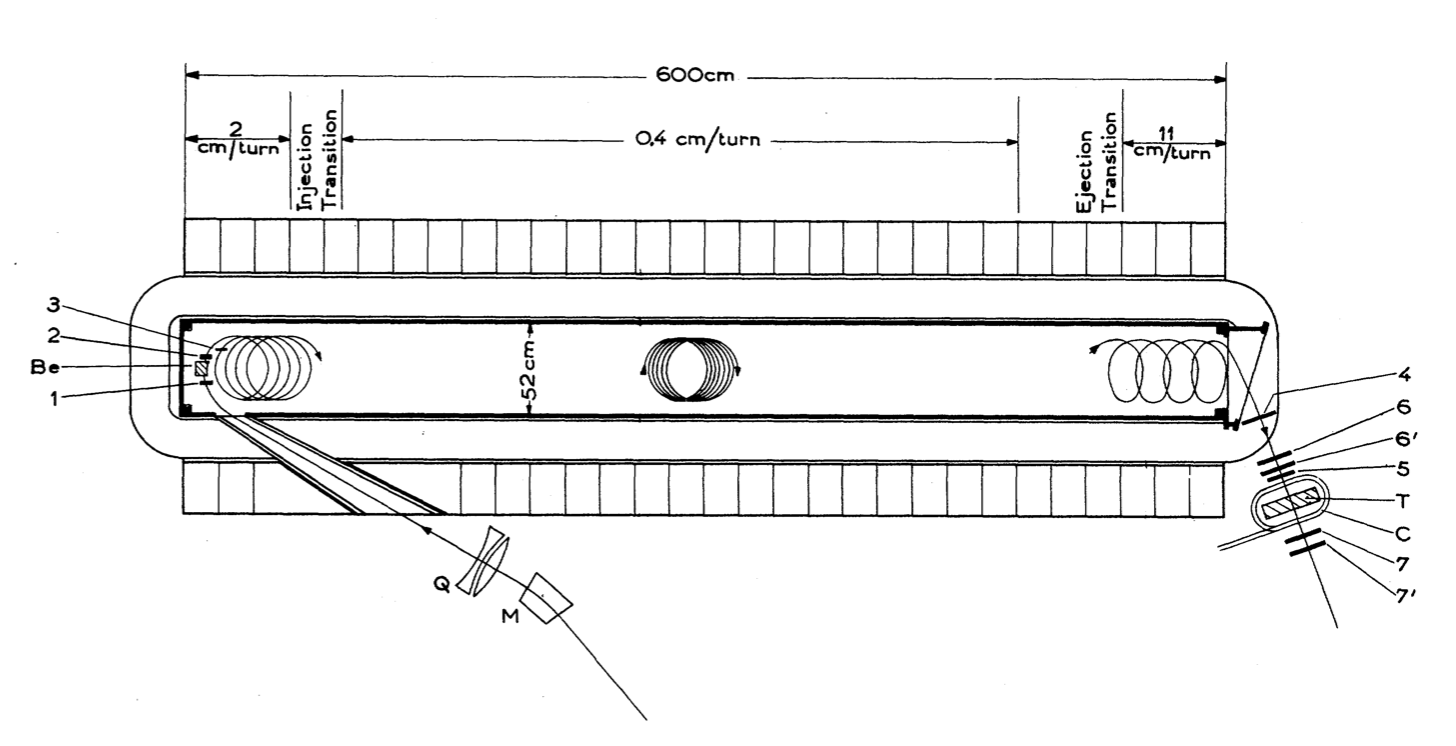
\includegraphics[width=0.9\linewidth]{fig/cern-i-diagram.png}
\caption{A diagram of the experimental setup in the first muon \gmtwo experiment at CERN from the original paper \cite{cern-i}. The muons enter from the lower left, go through the energy moderator to put the cyclotron radius at 19cm, drift and circle toward the ejection side of the magnetic field, escape from the magnet, stop in the fiducial block, and decay into an electron with momentum correlated to the spin direction. \label{fig:cern-i-diagram}}
\end{figure}

\subsection{CERN-II (1962-1968)}
The second iteration of \mugmtwo at CERN improved by a factor of 15 over the first.  CERN-II was the first \mugmtwo experiment to use the now familiar magnetic storage ring as shown in figure \ref{fig:intro-cern-ii-storage-ring}.  The storage ring design allowed the experimenters to measure $a_\mu$ directly as opposed to $g_\mu$ as explained near the beginning of the chapter. In order to store muons, the experiment injected a beam of protons which hit a pion production target.  A slice of the pion production phase space matched the momentum acceptance of the ring well enough to remain for several revolutions. The stored muons were mostly forward decays that lost a bit of energy and matched the ring's momentum acceptance.  The decay electrons curled inward to produce signals in electron counting detectors at a rate that modulated at the $\omega_a$.  The injected muons had a relativistic $\gamma$ of 12 which allowed the researchers to increase the observation time of muon spin precession to more than 130 $\mu s$.  The increased duration led to improved determination of $a_\mu$ to \ppm{270} \cite{47y-muon-g-2}.

\begin{equation}
\label{eqn:cern-ii-results}
a_\mu = 116\,616\,000 (31\,000) \times 10^{-11}
\end{equation}

\begin{figure}
\centering
\includegraphics[width=0.7\linewidth]{fig/intro-cern-ii-storage-ring}
\caption{
    The first muon storage ring used in the CERN-II experiment.  Pions were injected and a fraction of the forward decay muons matched the ring's momentum acceptance.  Those polarized muons orbited the ring until decaying into electrons which activated the detectors.  The electron rate signal was used to extract $a_\mu$.
    \label{fig:intro-cern-ii-storage-ring}    
}
\end{figure}

\subsection{CERN-III (1969-1976)}
The third CERN muon \gmtwo experiment was also the last.  A major innovation introduced in CERN-III was use of the so-called ``magic'' momentum. Observe equation \ref{eqn:full-omega-a}, the expression for spin precession in electromagnetic fields for a relativistic muon.

\begin{equation}
\label{eqn:full-omega-a}
\vec{\omega}_a = \frac{e}{m} \left[ a_\mu \vec{B} - \\
\left(a_\mu - \frac{1}{\gamma^2 - 1} \right) \\
\frac{\vec{\beta} \times \vec{E}}{c} \right]
\end{equation}

\noindent A muon beam at a very specific momentum, \pmagic, cancels the effects of radial electric fields which allows electrostatic focusing to be used on the muon beam instead of magnetic gradient focusing.  The perturbations from magnetic focusing were a large source of uncertainty in the previous experiment.  Another major innovation for the third CERN experiment was the use of pion injection instead of proton injection.  The measurement techniques of CERN-III were similar to CERN-II.  The new magnetic storage ring constructed for the experiment is shown in figure \ref{fig:intro-cern-iii-storage-ring}.  With the achieved improvements, the CERN team was able to drive down the uncertainty on $a_\mu$ to \ppm{7} \cite{47y-muon-g-2}, nearly a 40-fold improvement!

\begin{equation}
\label{eqn:cern-iii-results}
a_\mu = 116\,592\,300 (800) \times 10^{-11}
\end{equation}

\begin{figure}
\centering
\includegraphics[width=0.7\linewidth]{fig/intro-cern-iii-storage-ring}
\caption{
    The second muon storage ring used in the CERN-III experiment.  A radial line of \SI{7000}{\mm} is draw for scale.  Pions were again injected, though finer momentum selection was used which yielded higher spin polarization for the muons.  The electron counting detection method was similar to the technique used in CERN-II.
    \label{fig:intro-cern-iii-storage-ring}    
}
\end{figure}

\subsection{E821 at BNL (1984-2003)}
The most precise \mugmtwo experiment to date took place at Brookhaven National Laboratory (BNL). The experiment, E821 as it is labeled in high energy physics ledgers, pushed precision muon physics to a new level.  The precision goals for E821 demanded a 400-fold increase in statistics over its predecessor.  The magnetic storage ring was redesigned once again as is shown in figure \ref{fig:intro-e821-storage-ring}.  One critical improvement in the experiment was that E821 injected muons rather than pions, or protons.  Muon injection provided cleaner data earlier in each injection, and with an exponentially decaying number of muons, an early start time could lead to a huge rate improvement.  The experiment design also focused on improving the homogeneity of the magnetic storage field.  The aperture of the storage region was increased to facilitate a more uniform magnetic field across the muon storage volume.  Field measurement was also improved by implementing both a suite of stationary magnetometers outside of the storage region to continuously monitor magnetic field drift and a trolley outfitted with an array of 17 magnetometers to measure the field in the storage volume periodically.

In the end, the experiment nearly reached the initial goal of 350 ppb uncertainty on $a_\mu$, actually achieving 540 ppb uncertainty \cite{e821-prd}.  The E821 \gmtwo result was at odds with theoretical calculations.  Depending on which theoretical models were employed, the measurement was somewhere around $3.3\sigma - 3.6\sigma$ away from theoretical prediction, a statistical tension!

\begin{equation}
\label{eqn:e821-results}
a_\mu = 116\,592\,082 (55) \times 10^{-11}
\end{equation}

\begin{figure}
\centering
\includegraphics[width=1.0\linewidth]{fig/intro-e821-storage-ring}
\caption{
    The magnetic storage ring used in the BNL experiment.  The size of the ring was very similar to the CERN-II ring with a ``magic'' radius of \SI{7112}{\mm} for muon orbits.  In this storage ring, muons were injected directly into the storage ring.
    \label{fig:intro-e821-storage-ring}
}
\end{figure}

\section{The State of Theory} \label{sec:theory}

The theoretical contributions to \mugmtwo come from all corners of particle physics.  The typical division of contributions breaks them into QED, EW, QCD hadronic vacuum polarization (HVP), and QCD hadronic light-by-light (HLbL) as layed out in equation \ref{eqn:sm-contributions}. The QED correction is by far the largest. It is well understood though, so the uncertainty on the correction is small.  The next largest contributions to $a_\mu$ come from the QCD sector.  The QCD terms also dominate the uncertainty on the calculation.  The EW terms contribute a small, but well understood correction to $a_\mu$.  Figure \ref{fig:sm-contributions} in section \ref{sec:tension} is a visual overview of the corrections.  Theoretical progress for QED and EW corrections involves calculating increasingly intricate Feynman diagrams. The values are well understood though, so there is no need for a major theoretical effort.  The QCD contributions are trickier and represent a challenge to the theory community.

\begin{equation}
\label{eqn:sm-contributions}
a_\mu = a_{_{QED}} + a_{_{EW}} + a_{_{QCD-HVP}} + a_{_{QCD-HLbL}}
\end{equation}

\subsection{QED Effects} \label{s-sec:theory-qed}

The correction from QED interactions is the largest contribution to $a_\mu$.  Feynman diagrams provide a convenvient way to intuit some of the relevant effects.  All diagrams for QED are of the radiative correction type, shown in figure \ref{fig:qed-feynman-diagrams} (1\hbox{--}6).  These diagrams involve emission and recapture of a photon(s).  Another common type of diagram illustrates vacuum polarization interactions, shown in figure \ref{fig:qed-feynman-diagrams} (5\hbox{--}6), with the off-shell photon going through pair production and annihilation along its path.

\begin{figure}
\centering
\includegraphics[height=2.0\fdh]{fig/qed-feynman-diagrams}
\caption{
    Several examples of QED interactions illustrated as Feynman diagrams.  All six constitute radiative corrections which involve emission and absorption of photons. The last two are termed vacuum polarization effects, since the off-shell photon undergoes pair production.
    \label{fig:qed-feynman-diagrams}
}
\end{figure}

The QED corrections constitute over \SI{99}{\percent} of the total anomalous magnetic moment.  The QED corrections lend themselves to a perturbative approach represented by a power series in the QED coupling constant, $\alpha_{_{QED}}$.

\begin{equation}
\label{eqn:qed-correction-series}
a_{_{QED}} = \sum_n{A_n \left(\frac{\alphaQED}{\pi} \right)^n}
\end{equation}

\noindent
The first order term in the series is the leptonically universal Schwinger term, $a_{_{Schwinger}} = \frac{\alphaQED}{2\pi}$.  In terms of the measured value of $a_e$, the Schwinger term is $100.134\%$ of the measured value. And for $g_\mu$, the lowest order term is a slightly larger fraction of the total at $99.59\%$ \cite{codata}.  For the electron case, the higher order contributions are net negative which reduces the anomalous magnetic moment while further contributions are net positive for $a_\mu$. In both cases though, the Schwinger term dominates the corrections.

\begin{align*}
a_{e}   & = 115\;965\;218.091(26) \times 10^{-11} \\
a_{\mu} & = 116\;592\;080(63) \times 10^{-11} \\
a_{_{Schwinger}} & = 116\;120\;635.555(27) \times 10^{-11}
\end{align*}

For higher order terms in the QED correction, one can gain some intuition by investigating a vertex expression in the different mass limits.  First, consider the case of radiative corrections in which the radiated particles are light compared to the muon, $m_p \ll m_\mu$.  Equation \ref{eqn:qed-2nd-order-small-m} is a general expression for 2nd order terms in the small mass limit \cite{the-muon-g-2} where $n_p$ is the coupling order and $k_p < n_p$ is a possible enhancement to the logarithm term.

\begin{equation}
\label{eqn:qed-2nd-order-small-m}
\delta a_\mu^p \sim \left(\frac{\alpha}{\pi} \right)^{n_p} \\
\ln^{k_p} \left( \frac{m_\mu}{m_p} \right)
\end{equation}

\noindent
And, now consider the opposite case where $m_p \gg m$.  The expression changes to equation \ref{eqn:qed-2nd-order-large-m}.

\begin{equation}
\label{eqn:qed-2nd-order-large-m}
\delta_\mu^p \sim \left( \frac{\alpha}{\pi} \right)^{n_p} \\
\left( \frac{m_\mu}{m_p} \right)^2 \\
\ln^{k_p} \left( \frac{m_\mu}{m_p} \right)
\end{equation}

\noindent
The mass supression term can be understood as a result of the fact that these types of muon interactions with heavier particles requires helicity flips for the muon which add a $\frac{m_\mu}{m_p}$ factor and that vertex in the end is squared to yield an amplitude \cite{amm-of-muon}.

The two equations, \ref{eqn:qed-2nd-order-large-m} and \ref{eqn:qed-2nd-order-small-m}, offer insight into the difference between muon and elecron \gmtwo.  The electron mass is much smaller than the muon, so these are the type of higher order interactions that are enhanced in the muon \gmtwo.  Another major insight follows from the fact that electron interactions with large mass particles are suppressed.  The electron \gmtwo can be used to calculate a very precise value of $\alphaQED$ \cite{g-e-measurement}.

The contribution of QED effects have been calculated to 5 loops \cite{5-loop-qed}.  That includes more than 10,000 diagrams!  The correction from QED is well known and does not limit the certainty on the theoretical value.  The resulting contribution to \mugmtwo in total is

\begin{equation}
\label{eqn:qed-total}
a_\mu^{^{QED}} = 116\;584\;718.845(0.037) \times 10^{-11}.
\end{equation}

\subsection{EW Effects} \label{s-sec:theory-ew}

In general corrections due to the weak force are mass suppressed compared to QED corrections.  The lowest order and largest contribution to the weak corrections comes two diagrams, see figure \ref{fig:weak-lowest-order-diagrams}. One is similar to the Schwinger Diagram, the difference being that the photon propagator has been substituted for the Z boson.  The second entails emission of a muon neutrino, conversion to a W boson of the appropriate charge, and recapture of the neutrino.  The expression, equation \ref{eqn:weak-lowest-order} for the diagrams is calculated in \cite{the-muon-g-2} where the first term in brackets is derived for the W boson interaction and the second term for the Z boson.  The total contribution for the lowest order weak corrections is then \SI{194.9}{\times 10^{-11}}.

\begin{figure}
\centering
\includegraphics[height=\fdh]{fig/weak-lowest-order-diagrams}
\caption{The largest contributing diagrams from the weak interaction.  The muon in the left diagram goes off shell by emitting and re-absorbing a neutral Z or Higgs boson.  And, the muon in the right diagram converts to a $W^{-}$ ($W^{+}$ for $\mu^{+}$) and emits and re-absorbs a muon neutrino to conserve fermion number. \label{fig:weak-lowest-order-diagrams}}
\end{figure}

\begin{equation}
\label{eqn:weak-lowest-order}
a_\mu^{^{EW}} = \frac{G_F m^2}{8\sqrt{2}\pi^2} \\
\left[\frac{10}{3} + \frac{1}{3} \left(-5 + (1 - 4\sin{\theta_W}^2)^2 \right) \right]
\end{equation}

The next order in EW interactions might be expected to be nearly negligible.  Naively, they would be suppressed by a coupling factor of $\frac{\alpha}{\pi} \approx 0.002$, and so would amount to a small effect.  However, the contribution also gets an enhancement due to the large logarithm of $\log(m_Z/m) \approx 6.8$, and conincidentally many terms add coherently.  More difficulty arises as QCD effects arise within the weak boson propagators, which will not receive more than a mention here.  The total contribution from the second order weak diagrams ends up being \SI{-40}{\times 10^{-11}} \cite{the-muon-g-2}.  The total contribution to $a_\mu$ is given in equation \ref{eqn:ew-total}. 

\begin{equation}
\label{eqn:ew-total}
a_\mu^{^{EW}} = 154(2) \times 10^{-11}
\end{equation}

\subsection{QCD Effects} \label{s-sec:theory-qcd}

The QCD sector is undoubtedly the most difficult domain to calculate accurately and precisely in determining \gmtwo of the muon.  In general QCD calculations can be extremely difficult owing to the non-perturbative nature of many QCD problems, and \mugmtwo calculations are no exception.  Some calculations leverage effective low-energy perturbation theories, others chiral perturbation approaches, and others still utilize lattice calulations \cite{the-muon-g-2}.  The comprehensive approach involves both model-dependent calculations and model-independent contributions.  Sorting the bevy of contributions is a daunting task, fortunately muon \gmtwo theory reviews have already done just that for experimentalists \cite{the-muon-g-2, a-mu-harbinger, muon-g-2-blum, muon-g-2-hadronic-jegerlehner}.

\subsubsection{Hadronic Vacuum Polarization}

The general form of HVP is quite similar to the QED vacuum polarization described in section \ref{s-sec:theory-qed}.  The muon radiates a photon or emits another boson, and the newly created particle pair produces then annihilates before recapture with the muon, illustrated in figure \ref{fig:qcd-hvp-feynman-diagram}.  The difference being that in this case the pair production pulls from the hadronic sector instead of the lepton sector.  Such possibilities include: $\pi_0$, $\pi^+, \pi^-$, $\rho_0$, etc.  The size of the HVP correction is second only to the QED correction coming in at around \SI{7000}{\times 10^{-11}}.

\begin{figure}
\centering
\includegraphics[height=\fdh]{fig/qcd-hvp-feynman-diagram}
\caption{The basic diagram for hadronic vacuum polarization. \label{fig:qcd-hvp-feynman-diagram}}
\end{figure}

The hadronic vacuum polarization can be anchored to measurements of the hadronic cross-section.  The general method employed uses the integral relationship given as

\begin{equation}
\label{eqn:qcd-hvp-integral}
a_\mu^{hvp} = \frac{\alpha}{3\pi} \int_{s_0}^{\infty} \frac{ds}{s} \\
\frac{\sigma_{hadr}(s)}{\sigma_{point}(s)} a_\mu^{(1)}(s)
\end{equation}

\noindent
where $a_\mu^{(1)}(s)$ is the 1-loop contribution to $a_\mu$ from a neutral vector boson with mass $\sqrt{s}$, $\sigma_{hadr}$ is the $e^+e^-$ hadronic annihiliation cross-section, and $\sigma_{point}$ and further detail is given in reference \cite{amm-of-muon}.  With the data-driven method employed it is technically possible to extract the value exactly.  The reality of the calculation turns out to be difficult, since data from many different experiment needs to be well understood and combined to cover the whole spectrum.  

In a fairly recent theory review by Thomas Blum, et al \cite{muon-g-2-blum}, a recent value for the leading order and next order contributions combine to 

\begin{equation}
\label{eqn:qcd-hvp-total}
a_\mu^{^{QCD-HVP}} = 6824(42) \times 10^{-11}.
\end{equation}

\subsubsection{Hadronic Light-by-Light}

The general form for hadronic light-by-light (HLbL) contains more interaction vertices than HVP and, as is to be expected, therefore a smaller contribution to the total muon anomaly.  The core idea of hadronic light-by-light scattering is that the propagating the muon interacts with three photons and those photons interact with some sort of QCD loop which interacts with the external field.  The HLbL scattering is one of the most difficult $a_\mu$ contributions to calculate, because it cannot be anchored to experimental data using a dispersion relation like the HVP contribution \cite{the-muon-g-2}.

\begin{figure}
\centering
\includegraphics[height=\fdh]{fig/qcd-hlbl-feynman-diagram}
\caption{The basic diagram for hadronic light-by-light scattering.  The propagating muon interacts with a QCD black box which interacts with the disconnected photon diagram, i.e., the external field. \label{fig:qcd-hlbl-feynman-diagram}}
\end{figure}

The value is largely model dependent for $a_\mu^{^{QCD-HLbL}}$.  The most discussed model in reference \cite{amm-of-muon} uses a color extension allowing a large number of colors and includes constraints from chiral and short-distance QCD.  Other model calculations arrive at values up to 50\% different, but most are closer.  Many groups working in the field convened to establish the ``Glasgow Consensus'' as an agreed upon value for the correction \cite{e989-tdr}.  The consensus value is

\begin{equation}
\label{eqn:qcd-hlbl-total}
a_\mu^{^{QCD-HLbL}} = 105(26) \times 10^{-11}.
\end{equation}

\subsection{Beyond the Standard Model}

Consider the simplest extensions of the Standard Model where a new particle comes in analagous to a current particle.  A general argument can be made for an approximation of the size of the correction from such diagrams \cite{the-muon-g-2}.  For light particles where the new particle mass is less than the muon mass, $m_p < m_\mu$, the contribution is expected to have the following form:

\begin{equation}
\label{eqn:bsm-general-small-m}
\delta a_\mu \sim \left(\frac{\alpha}{\pi}\right)^{n_p} \left( \ln{\frac{m_\mu}{m_p}} \right)^{k_p}
\end{equation}

\noindent
where the exponent $n_p$ represents the loop order of the correction and the exponent $k_p$ is the possible logarithmic enhancement at the order.  Note that $k_p < n_p$, but not otherwise predictable.

The situation changes a bit when more massive particles are considered, because helicity flips must be accounted for.  In general those helicity flips add a unitless mass suppression term to the vertex function which is squared in the amplitude, so we get the following relation:

\begin{equation}
\label{eqn:bsm-general-large-m}
\delta a_\mu \sim \left(\frac{\alpha}{\pi}\right)^{n_p} \\
\left(\frac{m_\mu}{m_p}\right)^2 \\
\left(\ln{\frac{m_\mu}{m_p}} \right)^{k_p}
\end{equation}

\subsubsection{Supersymmetric Extensions}
With these two general estimates established, it is instructive to talk about a few specific types of corrections.  Supersymmetry (SUSY) is one proposed theory that can account for the deviation in $a_\mu$ with some tuning.  Supersymmetric contributions arise through smuon-neutralino and sneutrino-chargino conversions in loop diagrams such as figure \ref{fig:bsm-susy-diagrams}.  A general expression for contributions from SUSY is given in equation \ref{eqn:bsm-a-mu-susy} \cite{a-mu-harbinger}.  In equation \ref{eqn:bsm-a-mu-susy}, $\tilde{m}$ is the mass of the SUSY particle

\begin{figure}
\centering
\includegraphics[height=\fdh]{fig/bsm-susy-diagrams}
\caption{Two example diagrams of SUSY which would contribute to the anamalous magnetic moment. In the left diagram, the muon converts into the supersymmetric particles, the sneutrino, $\tilde{\nu}$ and chargino $\tilde{\chi}$, and back to the muon.  In the right diagram the muon undergoes a different supersymmetric interaction vertex to become a smuon, $\tilde{\mu}$, and a neutralino, $\tilde{\chi}^0$.  These one-loop diagrams are expected to be the largest contributors from minimal SUSY extensions of the SM. \label{fig:bsm-susy-diagrams}}
\end{figure}

\begin{equation}
\label{eqn:bsm-a-mu-susy}
\left|a_\mu^{SUSY}\right| \approx \\
\left(\frac{\alpha(M_z)}{8 \pi \sin^2{\theta_W}} \right) \\
\left( \frac{m_\mu}{\tilde{m}} \right)^2 \tan{\beta} \\
\left(1 - \frac{4\alpha}{\pi}\ln{\frac{\tilde{m}}{m_\mu}} \right) \\
\approx 130 \times 10^{-11} \\
\left(\frac{100 GeV}{\tilde{m}} \right)^2 \tan{\beta}
\end{equation}

The $\tan{\beta}$ enhancement can naturally be around 40 or 50.  The difference $a_{expt} - a_{theory} \approx 250 \times 10^{-11}$ puts the mass scale at $\tilde{m} \approx 500 \mathrm{GeV/c}$ for a SUSY effect the size of the muon anomaly tension.

\subsubsection{Radiative Extensions}
Another proposed theory, radiative mass models, can explain both deviations from \gmtwo and the ``unnaturally'' light mass of the leptons.  In this model the mass of the muon is generated by emission and absorption of an as yet unknown particle while it propagates, and the bare mass of the muon is zero.  The same new particle that provides mass would come in to the anomalous magnetic moment as an unnacounted for Schwinger-like term.  The size of the contributions in such a model are given in equation \ref{eqn:bsm-general-small-m}, and the diagrams in figure \ref{fig:bsm-radiative-diagrams} \cite{a-mu-harbinger}.

\begin{figure}
\centering
\includegraphics[height=\fdh]{fig/bsm-radiative-mass-diagrams}
\includegraphics[height=\fdh]{fig/bsm-radiative-a-mu-diagrams}
\caption{
    Example diagrams which would cause the mass of the muon and corrections to \mugmtwo.  The letters represent possible new scalar (S), pseudoscalar (P), and fermion (F) particles.
    \label{fig:bsm-radiative-diagrams}
}
\end{figure}

\subsubsection{Other Extensions}

Many other SM extensions have been proposed throughout the years.  See references \cite{a-mu-harbinger, the-muon-g-2, e989-tdr} for deeper discussions, but a few are listed here.  Dark photons are light, but very weakly coupling particles that could account for \mugmtwo.  Anomalous properties of the W boson, such as an anomalous magnetic moment or electric quadrupole, have been proposed as possible explanations.  Also, new gauge bosons models illustrate a possible avenue for anomalous \gmtwo.

Much of the phase space for the proposed standard model extensions has been ruled out by other measurements.  The LHC for instance has constrained the parameters in many SUSY models and other experiments have strongly restricted the possibility of dark photons.  However, most models are not completely ruled out, and the assay of possible solutions will need to be careful pruned and tuned by the theory community in the coming years.


\section{Experiment Versus Theory} \label{sec:tension}

From the experimental side, the combined average value from all measurements comes to 

\begin{equation}
\label{eqn:expt-a-mu}
a_{\mu,expt} = 116\,592\,082 (55) \times 10^{-11}.
\end{equation}

\noindent
Similarly, all individual theory contributions combine to the value given in equation \ref{eqn:theory-a-mu}.  \textbf{Note:} this value varies with different models, and the sum here is over the specific values listed in section \ref{sec:theory}.

\begin{equation}
\label{eqn:theory-a-mu}
a_{\mu,theory} = 116\,591\,802 (49) \times 10^{-11}
\end{equation}

\noindent
The difference between the two values is then

\begin{equation}
\label{eqn:diff-a-mu}
a_{\mu,expt} - a_{\mu,theory} = 280 (74).
\end{equation}

The discrepancy between theory and experiment given above is \SI{3.8}{\sigma}, and in the majority of models a discrepancy greater than \SI{3}{\sigma} persists.  The next step is to push the precision even further on both fronts, and turn a statistical tension into a \SI{>5}{\sigma} discovery (assuming constant central values).  The persistent discrepancy is a possible indication of new physics from beyond \tsm.

\subsection{Improvements in Theory}

All necessary theory work is in the QCD domain.  Currently, the QCD-HVP uncertainty dominates the theory uncertainty.  The value is expected to improve by adding additional cross-section data from Novosibirsk and BESIII experiments, and possibly through a lattice based approach \cite{muon-g-2-blum}.  

The next largest source of uncertainty comes from the QCD-HLbL correction.  There are two possibilities for reducing the uncertainty on the QCD-HLbL contribution.  One method is to make measurements of hard photon physics which the value can be anchored to similar to the QCD-HVP term \cite{muon-g-2-blum}.  Another possibility is calculation on the lattice which is already underway \cite{qcd-hlbl-blum-2016, qcd-hlbl-blum-2017}.  

The theory community aims to reduce the uncertainty on each contribution by a factor of two.  If these precision goals are met, the uncertainy on the theoretical value would be \SI{205}{ppb}.

\subsection{Improvements in Experiment}
The tension between past experiments and theory inspired a new wave of \mugmtwo measurements.  A new iteration of the \mugmtwo experiment is underway at Fermi National Accelerator Laboratory (FNAL). The experiment, E989, reuses the storage ring, superconducting coils, and various components from the BNL experiment.  The precision goal of E989 is an overall uncertainty of 140 ppb, likely pushing the tension to discovery levels. Additionally, a sister experiment has been proposed at J-PARC as a completely independent measurement of \mugmtwo with similar sensitivity to the BNL experiment.

\subsection{Summary}
The major values related to \mugmtwo are brought together for comparison in figure \ref{fig:sm-contributions}.  The three most recent experimental values are shown as vertical bars with the projected value from E989 also included as a dashed vertical line.  The theory contributions are grouped into QCD, EW, and QED sectors and split by order with the value shown in blue and the uncertainty shown in blue.

\begin{figure}
\label{fig:sm-contributions}
\centering
\includegraphics[width=1.0\linewidth]{fig/SM-contributions.pdf}
\caption{The visual depicts all different theoretical contributions to \mugmtwo with experimental values for comparison.  The value from each storage ring experiment is represented as a vertical line with the projected precision for E989 as a dashed line.  The size and uncertainty of various SM corrections grouped by interaction type are depected as bars extending onto the vertical axis. The most important point highlighted by the figure is that theory only needs to improve in the hadronic light-by-light and hadronic vacuum polarization sectors.}
\end{figure}

% Chapter details the E989 g-2 Experiment
\chapter {E989: The Muon \gmtwo Experiment} \label{ch:expt}

\section{Overview} \label{sec:expt-overview}

\subsection{The Muon Anomaly}

The principal result from the E989 experiment can be represented by a single expression in which the two frequency parameters are quantities measured very precisely by the \mugmtwo experiment and all other parameters are fundamental quantities precisely measured in other experiments.

\begin{equation}
\label{eqn:g-2-result-1}
a_\mu = \frac{\omega_a}{\omega_p} \frac{\mu_p}{\mu_e} \\
\frac{m_\mu}{m_e} \frac{g_e}{2}
\end{equation}

\noindent
The parameter $\omega_a$ is the anomalous spin precession frequency for the muon, and $\omega_p$ is the Larmor frequency for a free proton.  Both frequencies are induced by the same magnetic field and thereby exactly correlated. The analysis technique for $\omega_a$ is described in more detail in section \ref{sec:spin-precession}.  The $\omega_p$ analysis methods are further discussed in section \ref{sec:magnetic-field} and further still in chapter \ref{ch:field}.  The CODATA values \cite{codata} for the magnetic moment and mass ratios and reference \cite{g-e-measurement} for the g-factor of the electron are given below.

\begin{align}
\mu_p/\mu_e & = -658.210\;684\;8(54) \\
m_\mu/m_e & = 206.768\;284\;3(52) \\
g_e/2 & = 1.001\;159\;652\;180\;73(28) \\
\end{align}

An alternative expression for $a_\mu$ can be derived by using the relation $m_\mu / m_e = (g_\mu \mu_\mu) / (g_e / \mu_e)$.  

\begin{equation}
\label{eqn:g-2-result-2}
a_\mu = \frac{\mathcal{R}}{\lambda^+ - \mathcal{R}}
\end{equation}

\noindent
where $\mathcal{R} = \omega_a / \omega_p$ and $\lambda^+ = \mu_{\mu^+} / \mu_p$  which is measured in a muonium hyperfine splitting experiment \cite{muonium-hyperfine}.  Using the CODATA values \cite{codata}, the ratio computes to

\begin{equation}
\label{eqn:muon-to-proton-mu-ratio}
\lambda^+ = 3.183\;345\;139(10).
\end{equation}

% In both expressions for $a_\mu$, the value for $\omega_p$ represents magnetic storage field.  It must be the average magnetic field sampled by the muons though, so the magnetic field storage data needs to be properly weighted by the muon particle trajectories.

% \noindent With all the measurement values included, the equations for the $a_\mu$ become

% \begin{align}
% \Rightarrow a_\mu  & = -136\;254.919\;130\;2(75) \cdot \mathcal{R}
% \Rightarrow a_\mu  & = \frac{\mathcal{R}
% \end{align}

\subsection{Precision Goals}

The overall precision goal on $a_\mu$ is \SI{140}{ppb}.  \SI{100}{ppb} of uncertainty is allotted for statistics.  The systematic uncertainty limit on $\omega_a$ is \SI{70}{ppb}, and the systematic uncertainty limit on $\omega_p$ is equally \SI{70}{ppb}.  The individual terms summed in quadrature make up the entire uncertainty budget for the FNAL \mugmtwo experiment, nearly a four-fold improvment upon the precision of the previous experiment at BNL.  The statistical uncertainty goal can be achieved through recording $1.8\times10^{11}$ physics events \cite{e989-tdr}.  The plan to reach systematic uncertainty limits includes broad experimental improvements over E821 in hardware systems, data quality, and analysis techniques.  A subset of the improvement plans for the $\omega_p$ uncertainties is discussed in chapter \ref{ch:field}.

\subsection{Stages of the Experiment}

The \mugmtwo experiment can be broken into several stages.  In the subsequent sections the following stages are discussed:

\begin{itemize}[noitemsep]
\item{Muon Production}
\item{The Magnetic Storage Ring}
\item{Muon Injection}
\item{The Magnetic Field}
\item{Spin Precession}
\end{itemize}

\noindent
In this document, a brief overview of information in the E989 Technical Design Report (TDR) is given. See the original document, reference \cite{e989-tdr}, for further detail. 

\section{Muon Production} \label{sec:muon-production}

The first stage in an experiment that measures a property of muons is of course producing muons. The full chain of muon production goes from protons to pions to muons (to electrons).  Expert personnel at Fermilab have developed a new beamline to deliver muons to the \gmtwo experiment using much of the existing particle production and accelerator infrastructure.  The structure of the beamline is illustrated in figure \ref{fig:fnal-beamline-diagram}.

% \begin{figure}
% \centering
% \includegraphics[width=0.9\linewidth]{fig/muon-production-beamline}
% \caption{The accelerator beamline that delivers muons for E989.  Protons are accelerated to \SI{8}{\GeV/c} and bunched in the Recycler Ring.  Then the protons hit the pion production target and lithium focusing lens.  The pions propagate down the M1-M2-M3 line to the Delivery Ring where muons are bunched and delivered to MC-1, the \mugmtwo experimental hall, at \SI{12}{\second^-1} \cite{e989-tdr}. \label{fig:muon-production-beamline}}
% \end{figure}

\begin{figure}
\includegraphics[width=0.9\linewidth]{fig/fnal-beamline-diagram}
\caption{
    The diagram depicts all relevant FNAL beamlines for \gmtwo.  Protons begin accelerating in the Linac, continue in the Booster, and enter the Recycler Ring. In the Recycler the protons are bunched into high intensity, small time windowed groups.  The protons exit the Recycler and propagate down the P1, P2, and M1 beamlines to the secondary production target.  Positive secondaries (including pions which later yield muons) at \SI{3.1}{\GeV/c} are focused and transported down the M2 and M3 beamlines to the Delivery Ring.  In the Delivery Ring, the bunch propagates long enough to develop a timing separation between protons and the muons now populating the beam.  With the timing separation, the protons can be dumped and the muons can be extracted to continue along M4 and M5 to the \gmtwo storage ring. 
    \label{fig:fnal-beamline-diagram}
}
\end{figure}

Much of the FNAL accelerator infrastructure is reused for protons in new beamlines for the Muon Campus.  The protons begin in the Linac and accelerate through Booster.  From there, the protons continue into the Recycler Ring where they are manipulated into the high intensity bunches with short timing structure for \gmtwo.  Each proton bunch contains $\mathcal{O}(10^{12})$ protons with \SI{8}{\GeV} kinetic energy in time windows less than \SI{90}{\nano \second}.

The protons then propagate from the Recycler to the AP0 target where they collide with the target.  The collision produces $\mathcal{O}(10^9)$ positive secondary particles of which many are pions.  The secondary particles are focused via an electrostatic lithium lens into a secondary beam which goes through a momentum filter shortly after focusing.  Momentum selection yields a beam of \SI{3.1}{\GeV/c} with a momentum spread of \SI{\pm 0.10}{\frac{\delta p}{p}}.  The secondary beam then proceeds through P1, P2, M1, M2, and M3 beamlines into the Delivery Ring.  

The goals in the Delivery Ring are twofold.  First, the beam cycles around the Delivery Ring to create a spatial separation between the pions/muons and the more massive protons (slightly lower velocity for the same momentum), so that the protons can be removed.  Secondly, essentially all pions undergo in-flight weak decay into muons, so the outgoing beam is a very pure muon beam.  Four orbits around the Delivery Ring are enough to achieve both goals.

After the Delivery Ring, the now muon beam is extracted onto the path toward the \mugmtwo storage ring. Through the pion decay process the high and low energy muons have a net spin polarization (as discussed in section \ref{sec:muon-attributes}), and the beamline design acceptance is narrow around the filtered secondary energy of \SI{3.1}{\GeV/c}.  The muons produced at \pmagic by the pion beam are forward decays and thereby achieve a net spin polarization of around \SI{95}{\percent}.  A bunch of muons produced in the beamline is referred to as a ``fill''. These fills deliver $\mathcal{O}(10^{4})$ muons to the storage ring at an average rate of \SI{12}{\second^{-1}} \cite{e989-tdr}.

\section{The Magnetic Storage Ring} \label{sec:storage-ring}
The magnetic storage ring is the hardware for creating the main magnetic dipole field for the experiment.  The major components include three superconducting NbTi/Cu coils, a dozen ``C''-shaped flux return yokes in the form of steel blocks and plates, 72 high-purity steel poles, and a built-in adjustment kit with more than 1,000 tunable knobs.  Figure \ref{fig:magnet-cross-section} depicts a cross-sectional view of the magnet.  The full assembly is around \SI{3}{\meter} tall, \SI{15}{\meter} wide, and weighs more than 700 tons \cite{e989-tdr}.  The storage ring was designed with the objective of creating a magnetic field of \bmagic that is as uniform as possible over a toroidal storage volume with a major radius of \rmagic and a minor radius of \SI{4.5}{\cm}.

\begin{figure}
\label{fig:magnet-cross-section}
\centering
\includegraphics[width=0.9\linewidth]{fig/magnet-cross-section}
\caption{The cross-sectional view of the storage ring.  The magnetic field is produced by currents in the three superconducting coils.  The field strength is primarily determined by the geometry for the flux capture in the ``C'' yoke and pole surfaces.  The field can be adjusted locally in azimuthal using a built-in shim kit that includes top hat shims, edge shims, and wedge shims.}
\end{figure}

The magnetic field itself is generated by driving a current of a current of $5176\;A$ through all three superconducting coils.  Two of the coils reside at $R_{inner} = \SI{6677}{\mm}$, inside the storage radius. And, one of the coils resides at a larger radius, $R_{outer} = \SI{7512}{\mm}$.  The outer coil contains twice as much superconducting material as the two inner coils to generate approximately equal magnetic fields from inner and outer coils.  The inner and outer coils run with opposing currents to create a nearly vertical B-field in the space between them.  The overall strength of the magnetic field depends on the amount of ferric material around the coils to contain magnetic flux and concentrate the magnetic field.  By design, the return yokes and pole pieces draw in magnetic flux at the operational current to produce a magnetic field close to \bmagic in the opening of the ``C''.  To first approximation the magnetic field uniformity depends on the geometric uniformity of the gap between the two pole surfaces.  The precision machined, high-purity pole pieces provide two extremely flat parallel surfaces for optimal field uniformity.  The final dipole magnetic field uniformity at BNL was around \SI{\pm50}{ppm} \cite{e821-prd}. An effort was made to recreate the final state of the magnet assembly after the storage ring was transported to FNAL and re-assembled.  When initially powered though, the magnetic field had variations of around \ppm{1400} as shown in figure \ref{fig:initial-field}.

\begin{figure}
\label{fig:initial-field}
\centering
\includegraphics[width=0.9\linewidth]{fig/initial-dipole-field.png}
\caption{The initial dipole (average at azimuthal point) magnetic field when the storage field was first fully measured at Fermilab.  The peak-to-peak variation was around \ppm{1400}.  The umbrella-like sub-structure occurs every 10 degrees and corresponds to the changing gap between the slightly curved pole pieces.  The horizontal bands represent the average field value and the uniformity goals set forth by the experiment.  The band formed by the two dotted lines around the average value indicates the experimental goal of \SI{\pm 25}{ppm}.}
\end{figure}

The last essential piece of the magnetic storage ring is the intrinsic shim kit.  Shims in this context are objects made of ferric material with full azimuthal coverage of the storage ring which can be adjusted to improve the magnetic field uniformity locally. A collection of edge shims, wedge shims, and top hats provides over 1,000 knobs to make azimuthally localized changes to the magnetic field.
Magnetic field shimming is discussed in further detail in chapter \ref{ch:shimming}.

\section{Muon Injection} \label{sec:muon-injection}
To store muons in the strong vertical magnetic field, they must be transported through the backleg, fringe field region of the magnet.  The non-linear natural path through this region is non-trivial to predict or manufacture in the storage ring.  The solution to simplify muon injection was to create a homogeneous magnetic field volume to provide a predictable path into the storage region. This field region is created with a cleverly designed magnet, called the inflector, which is able to achieve a strong, nearly uniform vertical field over a small volume.  It is designed to contain much of its flux from leaking and perturbing the nearby precision magnetic field region.  The flux capture in the initial design was insufficient and it was later improved by adding a superconducting shield to the outside.  The inflector was designed to be adjustable over small angles which allowed the apparatus to optimize the nearly straight injection of muons. See figure \ref{fig:expt-inflector} for an image of the inflector and the beam trajectory through the inflector. \cite{e989-tdr, e821-prd}

\begin{figure}
\label{fig:expt-inflector}
\includegraphics[width=0.9\linewidth]{fig/expt-inflector}
\caption{The inflector diagram on the left illustrates the relative position of the inflector as the bridge from essentially outside of the storage field through to within the storage volume.  The trajectory of the beamline through the inflector area is depicted in the right plot.}
\end{figure}

Another problem arises after the injected muons complete their first orbit around the storage ring.  Moving on circular orbits in a nearly uniform vertical magnetic field, the muons would hit the downstream end of the inflector as they return to the injection point.  In figure \ref{fig:expt-kicker-correction}, the red track illustrates the problem and the blue track illustrates a optimally shifted orbit achieved after a fast kicker magnet imparts the necessary angular shift onto the muon bunch.  The kicker would ideally produce a flat magnetic field around \SI{275}{\gauss} with very sharp rise and fall times, $\mathcal{O}(10\;ns)$.  The real pulse shape deviates from a perfect square pulse and re-kicks muons with the residual magnetic field, but a newly designed kicker will help to prevent double kicking muons as they return to the kicker region on their second orbit of the ring \cite{e989-tdr}.  

\begin{figure}
\centering
\includegraphics[width=0.6\linewidth]{fig/expt-kicker-correction}
\caption{The figure illustrates the orbital mismatch problem with muon injection.  The red track illustrates the problem where the muons collide with the injection point, and the blue track illustrates the good orbit achieved after a perfect kick. \label{fig:expt-kicker-correction}}
\end{figure}

\section{Magnetic Field} \label{sec:magnetic-field}

The magnetic field is of critical importance to the muon \gmtwo experiment.  A magnetic field of \bmagic puts muons with ``magic'' momentum, \pmagic, into uniform circular motion at the ``magic'' radius of \rmagic.  The prescribed parameters lock a fraction, $\mathcal{O}(0.03)$, of the injected muons in circular motion until they decay.  To first order, the value of the magnetic field directly affects the rate of muon spin precession and cyclotron frequency.  In this light, the average magnetic field must be very well measured, since it folds directly into the determination of \wa.  To second order the magnetic field couples to the symmetries in the muon beam influencing the beam dynamics of the stored muons.  These deviations in beam dynamics make the analysis which matches muon trajectories with the magnetic fields along them more difficult, and therefore add uncertainty to the determination of the expectation value for $\omega_p$.

\subsection{The Field Expansion}

The ideal magnetic field for the experiment is entirely vertical at \bmagic with no deviations.  However, Maxwell's equations do not permit such a perfect field within a finite amount of space.  Reality requires that the experiment consider the quality of the central field and the effects of perturbations to the field which is conveniently done using a decomposition.  The expansion in equation \ref{eqn:field-expansion} introduces a common set of functions used in discussing magnetic field perturbations.  The expansion assumes the domain where $B_r \ll B_z$ and $B_\phi \ll B_z$ effectively reducing the 3D problem to a 2D problem.  The idea is to then expand inside the two-dimensional plane defined by a \SI{4.5}{\cm} circle in $r$ and $z$ at a single value of $\phi$.

\begin{align}
\label{eqn:field-expansion}
\begin{split}
B_z & = \sum_{n=0}^{\infty} \rho^n[a_n \sin{\phi} + b_n \cos{\phi}] \\
B_r & = \sum_{n=1}^{\infty} \rho^n[c_n \sin{\phi} + d_n \cos{\phi}] \\
\end{split}
\end{align}

\noindent
A visualization of the terms in the multipole expansion is given in figure \ref{fig:field-example-multipoles}.  Each multipole highlights a possible symmetry of the field over the 2D azimuthal slice of the storage region. The magnetic field is characterized in terms of multipoles where the dipole should average to \bmagic and all other terms should be minimized.

\begin{figure}
\includegraphics[width=\linewidth]{fig/field-example-multipoles}
\caption{The first seven multipoles in the field expansion, equation \ref{eqn:field-expansion}.  The first on the left is the dipole term which simply averages each point equally over the domain.  The next two are the normal and skew quadrupole which represent an inner to outer or top to bottom asymmetry in the field respectively.  The next four terms similarly represent further symmetries of the field.  They are termed: normal sextupole, skew sextupole, normal octupole, and skew octupole. \label{fig:field-example-multipoles}}
\end{figure}

\subsection{Determining $\langle \omega_p \rangle$}

The magnetic field is measured and monitored with a suite of magnetometers, custom pNMR probes. Chapter \ref{ch:field} discusses the analysis in depth, but a cursory overview is still provided here for completeness.  The field analysis combines pNMR measurements from three different major subsystems.  The trolley system is a cylindrical aluminum shell equipped to travel through the muon storage volume and an array of pNMR probes to measure the magnetic field in 2D azimuthal slices.  A full set of measurements from the trolley system is combined to produce a magnetic field map as a function of position over the entire muon storage volume.  While the trolley resides in the storage volume, the ring cannot accept muons, so a set of 378 stationary pNMR devices outside the storage volume called the fixed probe system monitor the magnetic field drift between trolley runs.  The final subsystem is the absolute calibration probe system which includes several, essentially independent devices from the rest of the pNMR probes.  The absolute calibration probes are used to correct for systematic effects that shift the proton precession frequency in the trolley and fixed probes.

All the field measurements combine to produce the magnetic storage field as a function of time and position, the target quantity from the field measurements.  Expression \ref{eqn:g-2-result-1} and \ref{eqn:g-2-result-2} actually need $\langle \omega_p \rangle$ which represents the average field experienced by muons.  The muon distribution, $M(\vec{r}, t)$, and the field values need to be integrated over the all muons that contribute to determination of $\omega_a$.  An appropriate expression for $\langle \omega_p \rangle$ is then given in equation \ref{eqn:field-omega-p-tilde}.

\begin{equation}
\label{eqn:field-omega-p-tilde}
\langle \omega_p \rangle = \int M(\vec{r}, t) \, \omega_p(\vec{r}, t)\; dt\;dV
\end{equation}

\section{Spin Precession} \label{sec:spin-precession}

It is essential that the storage ring contain muons in stable orbits until they decay into electrons.  The muons come in polarized in the injection direction.  While propagating around the storage ring, the polarization vector of the muons undergoes spin precession.

\subsection{Decay Characteristics}

Eventually the muons decay into electrons and neutrinos as discussed in section \ref{sec:muon-attributes}. Due to maximal parity violation in weak decays, the spin direction is correlated to the energy and momentum direction of the decay electrons.  In the rest frame (see figure \ref{fig:muon-decay-rest-frame}) it can be seen that accumulation of events with energy either less than half or greater than half the total possible energy would result in a signal (anti-)correlated with the spin direction.  Applying similar logic to the boosted spectrum (see equation \ref{eqn:muon-decay-lab-frame} and figure \ref{fig:muon-precession-fom}) is a key insight into the way \gmtwo works.

\begin{align}
\label{eqn:muon-decay-lab-frame}
n_{lab}(y) & = \frac{-8 y^2 + y + 1}{4 y^2 - 5y - 5} & a_{lab}(y) & = \tfrac{1}{5}(y - 1) (4 y^2 - 5y - 5)
\end{align}

\noindent
The point is still to choose a domain which has an integral maximizing the spin-momentum correlation for the events.  The expression for the statistical figure of merit for an event counting analysis is

\begin{align}
\label{eqn:expt-figure-of-merit}
NA^2 = \int_{y_{thresh}}^{1} n(y) a^2(y) \;dy.
\end{align}

\noindent
The ideal energy threshold in this case is $0.4\times$\pmagic$ = $ \SI{1.24}{\GeV/c} as illustrated in figure \ref{fig:muon-precession-fom}.  The connection of muon spin to the decay electron energy is now established, so the last step in measuring the spin precession requires a technique to measure the energy and the birth time of emitted electons. \cite{e821-prd}

\begin{figure}
\centering
\includegraphics[width=1.0\linewidth]{fig/muon-precession-fom}
\caption{The plot depicts an unnormalized probability distribution for the number of decay electrons in the boosted lab frame, and similarly the fractional asymmetry as a function of the electron energy where the energy is represented as a fraction of the maximum possible electron energy from a muon momentum at \pmagic. Alongside the distributions, there is also a plot of $NA^2$ which is the statistical figure of merit for measuring decay events and maximizing the signal from the spin correlation. \label{fig:muon-precession-fom}}
\end{figure}

\subsection{Electron Calorimetry}

A suite of calorimeters arranged around the inner radius of the storage ring measure properties of the decay electrons.  The decay electrons always have less energy than the magic momentum, and so must curl inward on a smaller orbit radius than the storage orbit radius of the initial muon.  The trajectory of a typical decay electron is shown in figure \ref{fig:omega-a-decay-electron-trajectory}.  The trajectory of the electrons intersects with a calorimeter, at least the higher energy electrons anyway. The higher energy electrons have a wider trajectory similar to the parent muon and hit the calorimeters head on.  Lower energy electrons have a sharp trajectory which can curl inward between calorimeter stations.

\begin{figure}
\centering
\includegraphics[width=1.0\linewidth]{fig/omega-a-decay-electron-trajectory}
\caption{
    The figure shows a few typical decay electron trajectories.  The muon decays into an electron with lower momentum which by necessity takes a path with a smaller radius of curvature.  The electron curls inward into one of 24 calorimeter blocks around the inner radius of the storage ring. 
    \label{fig:omega-a-decay-electron-trajectory}
}
\end{figure}

The calorimeters establish a time and energy for each detected electron.  The device consists of a 6x9 array of $\mathrm{PbF_2}$ crystals each with a physically smaller array of geiger-like photon counting hardware called a silicon photomultiplier (SiPM).  Segmenting the detector decreases the likelihood of two decay events occurring simultaneously in the same measurement channel.  These double events are referred to as pileup and were a major source of uncertainty in E821.  The incoming electron produces thousands of \v{C}erenkov photons per \SI{}{\GeV}.  The photons collect at the opposite end of the crystal where they activate SiPM channels.  The subsequent pulse undergoes signal shaping, digitization, and a pulse fitting analysis routine to determine the energy and the time of the electron decay event.  

\subsection{Determining $\omega_a$}

The signal for the anomalous muon precession frequency manifests in histogramming electron detection events with energy above a cutoff threshold into time bins. The so-called ``wiggle'' plot exhibits clear oscillations which through careful systematic analysis result in a precise value for the anomalous precession frequency, $\omega_a$.  The muons undergo decay into electrons at an exponential rate, and the energy distribution of those electrons changes depending on the direction of the spin vector.  As the spin vector precesses, the number of decay electrons measured above threshold also fluctuates as shown in figure \ref{fig:omega-a-wiggle-plot}.  The basic model for the precession frequency signal is then given as 

\begin{equation}
\label{eqn:omega-a-signal}
N(t, E) = N_0(E) e^{-t/\tau_\mu} \left[ 1 + A(E) \cos(\omega_a t + \phi_0(E))\right]
\end{equation}

where $N_0$ is the total number of muons above threshold at time zero, $\tau_\mu$ is the effective muon lifetime, $A(E)$ is the total asymmetry of muons above threshold, and $\phi_0(E)$ is the phase of the spin vectors at $t_0$ for the fit.  A five parameter fit using equation \ref{eqn:omega-a-signal} yields the anomalous spin precession for muons.  The distribution and fit is depicted in figure \ref{fig:omega-a-wiggle-plot}.

\begin{figure}
\centering
\includegraphics[width=0.9\linewidth]{fig/omega-a-wiggle-plot}
\caption{
    The histogram is from the E989 TDR, reference\cite{e989-tdr}.  It shows the number of electron decay events above threshold as a function of time.  The oscillations seen on top of the exponential decay correlate to the spin precession of the muons as they propagate around the storage ring.  The number of high energy decays is enhanced as the spin aligns with the momentum and decreased when the spin anti-aligns with the momentum vector. 
    \label{fig:omega-a-wiggle-plot}
}
\end{figure}

\chapter{Field Measurement} \label{ch:field-meaurement}

\section{Measurement Requirements}

The \mugmtwo experiment allots \SI{70}{ppb} total uncertainty for the the field measurement.  The uncertainty comes in many flavors that are enumerated in source\cite{e989-tdr} and summarized in table \ref{tab:field-uncertainties}.  The uncertainty constraints help paint the picture for the next section which walks through the overall field measurement technique.

\begin{table}[h]
\label{tab:field-uncertainties}
\caption{Magnetic Field Uncertainty Budget}
\centering
\begin{tabular}{l c}
    \hline
    \multicolumn{1}{c}{Source} & Uncertainty [ppb] \\
    \hline
    Calibration of fixed probes   & 35 \\
    Calibration of trolley probes    & 30 \\
    Trolley measurements of $B_0$    & 30 \\
    Interpolation with fixed probes  & 30 \\
    Muon distribution                & 10 \\
    Inflector fringe field           & -  \\
    Time dependent external B fields & 5  \\
    Other sources                    & 30 \\
    \hline
    Total $\delta \omega_p$          & 70 \\
    \hline
\end{tabular}
\end{table}

\section{Hardware Design} \label{sec:field-measurement-technique}

The \gmtwo experiment has stringent requirements on the measurement uncertainty of the magnetic field value.  Stringent enough to aim for an entire error budget on the field uncertainty which is systematic.  Each individual measurement needs to be precise enough that the statistical error of the combined field value is negligible.  This puts an uncertainty limit of around \ppb{10} \note{where is this listed?}.  The field measurement technique is custom pulsed proton nuclear magnetic resonance (pNMR), a reprise of the measurement technique used in E821.  The probes were designed to have a very high Q-value resonance at the expected resonance frequency of \SI{61.79}{\MHz}.

\subsection{Proton NMR Signal}

The essence of a pNMR measurement is frequency measurement of another type of precession, proton precession.  The source of the pNMR signal is a volume of material with a population of quasi-free protons.  The active volume is polarized in the direction of a large field, in the case of \gmtwo a \bmagic field in the vertical direction.  A secondary field rotating in the orthogonal plane at a frequency approximately equal to the expected precession frequency of B-magic.  The intended effect of the secondary field is intuitively understood in the rotating reference frame.  In the rotating frame the vertically (z-direction) polarized protons experience an orthogonal (y-direction) field which rotates them into the orthogonal plane (x-y plane).  In the lab frame the polarized protons continue to precess at a rate proportional to the strong vertical field.  Precession in the orthogonal plane produces an induction signal in a nearby pickup coil which is subsequently digitized and analyzed.  A result of robust frequency analysis on the pNMR signal serves as high precision field proxy for \gmtwo experiment.

\subsection{Free Induction Decays}

The polarized protons involved in the FID evolve according to the Bloch Equations.  An ordinary differential equation that couples magnetization and field in different dimensions.

\begin{align} 
\begin{split}
\label{eqn:fid-bloch}
\frac{dM_x(t)}{dt} & = \gamma (\mathbf{M}(t) \times \mathbf{B}(t))_x - \frac{M_x(t)}{T_2} \\
\frac{dM_y(t)}{dt} & = \gamma (\mathbf{M}(t)\times \mathbf{B}(t))_y - \frac{M_y(t)}{T_2} \\
\frac{dM_z(t)}{dt} & = \gamma (\mathbf{M}(t) \times \mathbf{B}(t))_z - \frac{M_z(t) - M_0}{T_1}
\end{split} 
\end{align}

The ideal FID waveform from a pure field value and perfect $\pi/2$ pulse can be solved exactly from the differential equations.  The resulting equation, \ref{eqn:ideal-fid}, exhibits the primary characteristics of an FID, a sinusoid term representing the proton precession and an exponential decay envelope representing the $T_1$ relaxation.  Figure \ref{fig:fid-ideal-waveform} exhibits the waveform of an ideal FID.

\begin{equation}
f(t) = e^{-t/T_1} \sin(\omega t - \phi_0)
\label{eqn:ideal-fid}
\end{equation}

\begin{figure}
\label{fig:fid-ideal-waveform}
\centering
\includegraphics[width=0.5\linewidth]{fig/fid-ideal-waveform}
\caption{The figure shows an idealized FID waveform. Functionally, the waveform is a sinusoid muliplied with an exponential decay between at some initial time.  It represents the signal from a perfect $\pi/2$ to a perfect pNMR probe.}
\end{figure}

In a realistic situation, the FID signal is a summation over varying field values, and the signal bears strong deviations from the ideal FID form.  Nevertheless, the ideal signal is a valid testing bed for frequency extraction algorithms.  Examples of measured FIDs are shown in figure \ref{fig:fid-measured-waveforms}.

\begin{figure}
\label{fig:fid-measured-waveforms}
\includegraphics[width=0.9\linewidth]{fig/fid-measured-waveforms}
\caption{Two examples of measured FIDs are shown above. The image on left was measured with a test setup at CENPA (University of Washington), and the waveform on the right is an example from the E821 experiment fixed probe system.}
\end{figure}


\subsection{Probe Design}

The core design of the pNMR probes was based on the design from the previous experiment. Each probe consists of two pickup coils, a teflon backbone, a tunable capacitor, an alimunimum shell, and a \SI{5}{\meter} BNC cable.  One coil is used to inject the $\pi/2$ pulse which rotates the protons into the orthogonal plane, and the other is the induction coil used to produce the pNMR precession signal.  The capacitor allows the probe resonance to be tuned finely.  The aluminum shell allots some capacitance to the probe and shields against external effects.

\begin{figure}
\label{fig:field-pnmr-probe-design}
\includegraphics[width=0.9\linewidth]{fig/field-pnmr-probe-design}
\caption{\todo{caption}}
\end{figure}

The field team at \uw iterated on the probe design making several improvements.  One of the improvements was in the robustness of the connection to the BNC cable.  The new design used a crimp connection to secure the cable to provide a more robust connection.  Another improvement was the design of the tuning capacitor.  With the new design, the tuning of the probe can be done without removing the outer shell.  Removing the shell the has the chance of damaging the innards of the probe, and minimizing removals makes tuning easier, faster and safer overall.  Another major improvement is the material used as protonated, polarized volume.  The new design replaced the water and copper sulfate volume with a petroleum jelly.  The water design was seen to cause corrosion in many of the E821 probes, so the new design should alleviate those concerns and allot the provide a longer, stable lifetime.

\todo{Get resources from Martin, have him proofread}

The pNMR probes are used in two fairly different systems to measure the field.  The \fps comprises 378 probes located all around the storage ring to achieve thorough field coverage.  The actual volumes occupied by the fixed probes are outside of the muon storage volume.  The purpose of the \fps is to monitor the drift of the field at different locales around the ring.  The other system to use the pNMR probes is the Trolley System. The Trolley contains an array of 17 probes which carve out an azimuthal plane in the muon storage volume.  The trolley runs on rails all around the ring and uses the pNMR probes to measure the magnetic field in the muon storage region.  

\subsection{Fixed Probe System (FPS)}

The pNMR probes signal requires a parallel system of controlled electronics equipment.  The E989 reprised the NMR pulser design from the E821 experiments.  In order to generate a pNMR signal, the first phase is generating a $\pi/2$ pulse to rotate the protonated volume.  The $\pi/2$ pulse is generated by TTL input trigger which is tunable from \SIrange{4}{7}{\micro\second}.  After the the $\pi/2$ pulse, the free induction decay signal is mixed down against a very stable, \SI{61.74}{\MHz} rubidium frequency source.  The resulting signal feeds through a lowpass filter with $f_0$ of around \SI{200}{\kHz} \todo{check value}.  The filtered signal is fed into a waveform digitizer and recorded at a sampling rate of \SI{10}{\MHz} and samplingt depth of $16\;bits$.  The digitized waveform contains frequency information that represents the magnetic field.

\todo{signal diagram of the fixed probe system}

\subsection{Trolley System (TS)}

The trolley measures the magnetic field in the muon storage volume.  It cannot measure while muons are injected though, so there is a naturally trade-off between measuring the 3D storage field with the trolley and interpolating the field with the fixed probe system while the muon beam is being delivered.  The trolley uses an array of 17 of the standard pNMR probes as shown in figure \ref{fig:field-trolley-probe-array}.

\begin{figure}
\label{fig:field-trolley-probe-array}
\includegraphics[width=0.6\linewidth]{fig/field-trolley-probe-array}
\caption{An image of the trolley module itself is shown on the left.  The trolley rides along a rail system inside the vacuum chambers.  It traverses the muon storage volume.  The probes are arranged at three different radii as shown in the figure on the right.  The probe arrangement facilitates the multipole analysis used on the field data.}
\end{figure}

\subsection{Fluxgate Magnetomete (FM))}

\todo{add short section on fluxgates}

\subsection{Absolute Calibration Probes}

The frequencies measured by the pNMR probe systems in the ring are used to construct a 3D map of proton frequencies in the muon storage volume.  The frequency is a direct proxy for the field, but not an absolute value.  To bring the measurement back to an absolute proton precession precession, the absolute field value, there must be a correction applied.  The size of that correction is determined by the absoluate calibration system.

Several unique probes are used as independent determinations of the free proton resonance frequency.  E989 will make absolute field calibration measurements with the E821 probe, a newly design water probe from UMass, and a $\mathrm{^3He}$ probe with very different systematics. The probes are designed to minimized systematic effects that shift the free proton frequency.

\begin{equation}
\label{eqn:nmr-effects-model}
\omega_{probe} = (1 - \sigma(H_2 O, T) - \delta_b - \delta_p - \delta_s) \omega_p
\end{equation}

The model for free proton frequency includes corrections for geometric effects of the probe structure.  These geometric effects couple into the overall capacitance of the probe which can shift the resonance frequency.  They are minimized by using shapes with known ideal factors, cylinders and spheres.  The overall probe design must also minimize the magnetic perturbations from ferromagnetic and paramagnetic materials.  As such each component is vetted independently before becoming a part of the absolute probe.  The measurement also needs to control the environment of the probe and make a temperature correction.

\todo{ask d-flay and midhat if this is general or should split into he3/water probes}

The relative relationship between the absolute probe proton frequency and the pNMR probe frequency is done the so-called plunging probe system.  The plunging probes are brought into the same volume of field measured and corrected by the absolute probe to establish a transfer calibration from the absolute probe, which does not enter the storage ring, to a system which has a ring entry point.  The plunging probes are inserted into an azimuthal slice of the storage volume, plunged if you will.  The plunging probe is moved by a motor stage to be as near to each trolley probe as possible.  In this way, the free proton resonance from the absolute probe can propagate to the pNMR monitor probes used to measure the \gmtwo magnetic field.

\section{Field Reconstruction Technique}

The algorithms for field construction are not manifest, and they must be designed and refined by the field team over the coming months and years.  In this light, the contributions cannot be talked about in more than general terms.  The 3D field is re-measured periodically, and only the most recent one contributes to the field definition. The most general form for the field is then

\begin{equation}
\label{eqn:field-construction}
\vec{\omega}(\vec{r}, t) = \sum_n \Theta(t - t_n) \\
\Big[ \vec{\omega}_{n}(\vec{r}) + \delta\vec{\omega}(t) \Big]
\end{equation}

where we have a 3D field term, $\vec{\omega}_{n}(\vec{r})$, to serve as the base, and an interpolation term, $\delta \vec{\omega}(\vec{r}, t)$, to improve precision between runs. The last step in the field deliverable is calibrating the field determined by the trolley using the plunging probes and the absolute probes.

\begin{equation}
\label{eqn:field-calibration}
\omega_0(\vec{r}, t) = \alpha (\omega(\vec{r}, t) + \delta \omega_{cal})
\end{equation}

The process of defining the \gmtwo storage field begins with the trolley system.  The trolley system takes a run and uses the data to define the 3-dimensional magnetic field at the time of the run, $\vec{\omega}(\vec{r}, t_i)$.  Between trolley runs, measurements from the fixed probes and the fluxgates are used to interpolate the field changes.  The field changes affected from the fixed probes should be a function of time only, $\delta \vec{\omega}_{fps}(t)$.  And, likewise the contributions to interpolation from the fluxgates should be a function of time only, $\delta \vec{\omega}_{fm}$.  Stitching all the pieces together we arrive at equation \ref{eqn:field-construction}.

\subsection{3D Field}

The latest data from a full trolley run, a set of measurements encompassing all azimuthal locations in the storage ring, serves as a fundamental definition of the field.  The trolley continuously cycles through the 17 probe array while taking measurements at \SI{34}{\Hz}, two full cycles per second.  The full run process takes over an hour which yields at least 7,200 measurements with the full array.  Define the measurements as a 17xN matrix, $\vec{\Omega}_{tp}$. Each field measurement is accompanied by multiple complimentary location measurements.  The full suite of trolley measurements is then used to define a three dimensional magnetic field.

\begin{equation}
\label{eqn:field-base}
\vec{\omega}_{n}(\vec{r}) = g(\sum_{i}f_i(\vec{\omega}, \theta))
\end{equation}

The allotted uncertainty for constructing $\vec{B}_0$ is \SI{30}{ppb}.  Using the assumption of $\sim 7200$ measurements per trolley run, the accuracy of the field map can be estimated.  In this case, the average spacing between trolley measurements is about \SI{1}{mm}.  The accuracy of the position determination is similar in magnitude, \SI{\sim 1}{mm}, a little better.  Under these assumptions, the necessary accuracy at each point is 

\todo{finish error write up}

\subsection{Interpolation}

Between trolley runs, the field still needs to be well known.  The uncertainty budget on the interpolation of the 3D field is \SI{30}{ppb}.  There are two potential contributions to the field interpolation

\begin{equation}
\label{eqn:field-interpolation}
\delta \vec{\omega}(t) = \delta \vec{\omega}_{fps}(\vec{f}, t_i) \\
+ \delta \vec{\omega}_{fm}(\vec{x}, \vec{b}, t_i)
\end{equation}

The fixed probes provide one data source used for interpolation.  There are 378 fixed probes around the ring which measure the field at \SI{\sim 1}{\Hz}.  An pNMR frequency is extracted from each probe, and the data it timestamped.  A algorithm for field interpolation will be designed using all fixed probe measurements since the last trolley run, such as

\begin{equation}
\label{eqn:field-interpolation-fps}
\delta \vec{\omega}_{fps}(t) = \sum_{t_i = t_n}^{t_i < t} \delta f(\vec{f}, t_i)
\end{equation}

The second arm of field interpolation is the fluxgate magnetometers.  The fluxgates measure the transient field at high rates, \SI{\sim 1}{\kHz}.  There are three fluxgate sensors in the array which can be moved around the ring to monitor local field transients at multiple locations.  The transient fields measured in the fluxgates need to be well correlated and calibrated with the fields measured in the fixed probes, but they are a potentially powerful tool for discerning moderate frequency transients in the field, such as \SI{15}{\Hz} or \SI{60}{\Hz}.  Each sensor needs a human defined probe position vector, and provides a vector magnetic field value and time.  If they transient fields are small, as they are expected to be, the fluxgate could be used to simply place a limit on the effect of transient fields.

\begin{equation}
\label{eqn:field-interpolation-fm}
\delta \vec{\omega}_{fm}(t) \\
= \sum_{t_j = t_n}^{t_j < t} \delta f(\vec{x}, \vec{b}, t_j)
\end{equation}

\subsection{Calibration}

Calibration is the the final step in producing an absolute field map.  The calibration flows down from the absolute probe in two stages.  The absolute calibration probe and the plunging probe both measure the field in a certain location of a monitored and understood field.  The relationship is parameterized by a model.  One possible model is the linear model given in equation \ref{eqn:field-calibration-abs-pp}.

\begin{equation}
\label{eqn:field-calibration-abs-pp}
\omega_{absolute} = \alpha(\omega_{plunging} + \delta \omega_{absolute})
\end{equation}

The second stage of calibration is similar to the first.  The plunging probe measures the field in approximately the same volume as the trolley probes.  The calibration relationship can then be transferred in a similar way.  The linear model, equation \ref{eqn:field-calibration-pp-fp}, is given as an example.

\begin{equation}
\label{eqn:field-calibration-pp-fp}
\omega_{plunging} = \beta(\omega_{trolley} + \delta \omega_{plunging})
\end{equation}

Bringing the field map and the calibration together, one arrives at an expression for the field map as a function of time, the field team deliverable quantity.

\begin{equation}
\label{eqn:field-omega-p}
\omega_p(\vec{r}, t) = \alpha 
\Big [ 
\beta (\omega_0(\vec{r}, t) + \delta \omega_0) + \delta \omega_{pp}
\Big ]
\end{equation}

\subsection{Beam Convolution}

There is one final step in turning all of the pNMR probe measurements from the field into the value that feeds into the function for $a_\mu$.  The field function itself is not important.  The field value needs to be converted into the average field experience by the stored muons.  The muon distribution is measured by Fiber Harp Detectors and the reconstructed using the Tracker Detectors\cite{e989-tdr}.  The muon-weighted raw proton precession frequency can be determined by convolving the field team and beam team deliverables.

\begin{equation}
\label{eqn:field-omega-p-tilde}
\tilde{\omega}_p = \int M(\vec{r}, t) \times \omega_p(\vec{r}, t) dV
\end{equation}

\chapter{FID Analysis} \label{ch:fid-analysis}

The FID signals generated in the pNMR probes contain frequency information that represents the effective field seen by protons in the probe's active volume.  During a measurement the net polarization vector of the protons rotates into the plane orthogonal to the magnetic field, then the protons undergo Larmor precession due to the field.  The average precession frequency of the protons immediately after the $\pi/2$ pulse is the target of FID analysis.

\section{Frequency Extraction Methods}

An example FID is given in figure \ref{fig:fid-example-waveform}.  The main characteristics of the signal are amplitude oscillations at the Larmor frequency of the proton sample, and a decaying envelope function returning the signal back to the baseline noise.

\begin{figure}
\centering
\includegraphics[width=0.7\linewidth]{fig/fid-example-waveform}
\caption{
    The example highlights the key characteristics of an FID waveform.  The waveform starts abruptly after the $\pi/2$ pulse, oscillates at the Larmor frequency, and diminishes with some decaying envelope function which is often nearly exponential.
    \label{fig:fid-example-waveform}
}
\end{figure}

\noindent
As in most data analyses, the first step is cleaning and characterizing the data.  In the case of FIDs, the process begins with removing the baseline (and trend in some cases).  The next step in data preprocessing is determination of the start time and stop time of the useful FID signal within the frame of the entire recorded waveform.  The baseline value is calculated using an initial segment of the waveform which is free of signal.  The signal duration is computed using the maximum amplitude around the signal baseline and applying an amplitude threshold to find the first and last sections of the waveform with an envelope above that threshold.  After the FID has been characterized, it is ready for frequency extraction.

% \note{if time, add flow images for data pre-processing}

\subsection{Zero Crossing Method (ZC)}
The simplest method for determining the FID frequency involves counting zero crossings of the signal.  The technique was used in the previous \mugmtwo experiment in a hardware implementation, and has been re-implemented in software for E989.  The zero crossing method is a time domain algorithm which counts all zero crossings in the signal ($N$), then determines the time of the first and last zero crossing using a polynomial fit ($t_i$ and $t_f$).  The FID frequency is then given by equation \ref{eqn:fid-freq-zc}.

\begin{equation}
\label{eqn:fid-freq-zc}
\omega_{zc} = \frac{1}{4 \pi}\frac{N - 1}{t_f - t_i}
\end{equation}

\noindent
The method prevents double counting of zeros due to noise fluctuations by requiring the signal cross an amplitude threshold before allowing another countable zero crossing.  The threshold is referred to as the hysteresis threshold, and the concept is illustrated in figure \ref{fig:fid-freq-zc-hysteresis}.

\begin{figure}
\centering
\includegraphics[width=0.7\linewidth]{fig/fid-freq-zc-hysteresis}
\caption{
    The figure illustrates aspects of the zero crossing frequency determination technique.  The timing of first and last zero crossings are determined using a local polynomial fit which is represented by the orange and green lines.  The number of zeros is incremented at a sign change, then frozen until the signal amplitude goes outside of the dotted gray lines.  Using such a threshold is essential to the method as it suppresses erroneous zero counts.
    \label{fig:fid-freq-zc-hysteresis}
}
\end{figure}

The uncertainty associated with the zero crossing technique can be examined with a standard error analysis formulation given in equation \ref{eqn:uncertainty-analysis} \cite{error-taylor}.

\begin{equation}
\label{eqn:uncertainty-analysis}
\frac{\delta f}{f} = \frac{1}{f} \sum_{i} \\
\sqrt{\left| \frac{\partial f}{\partial x_i} \right|^2 (\delta x_i)^2}
\end{equation}

\noindent
In the case of the zero crossing algorithm, equation \ref{eqn:uncertainty-analysis} yields:

\begin{equation}
\label{eqn:fid-ferr-zc}
\frac{\delta \omega}{\omega} = \\
\sqrt{
    \left( \frac{\delta N}{N} \right)^2 +
    \left( \frac{\delta t_i}{t_f - t_i} \right)^2 + 
    \left( \frac{\delta t_f}{t_f - t_i} \right)^2
    }.
\end{equation}

\noindent
For the first term in equation \ref{eqn:fid-ferr-zc}, larger values of $N$ lower the uncertainty, and for the next two terms longer FID durations, $t_f - t_i = \Delta t$, lower the uncertainty.  By using a proper hysteresis threshold, $\delta N$ is suppressed to effectively zero. The start and stop times for the FID are determined by using a cubic fit around the first and last zero found in the algorithm.  By assuming the waveform is an ideal FID (see equation \ref{eqn:ideal-fid}) and expanding around the zero points, one finds that 

\begin{equation}
\label{eqn:error-on-ti-tf}
\delta t = \frac{\delta y}{A \omega} = \frac{1}{S \omega}
\end{equation}

\noindent
where $\delta y$ is the amplitude noise on the time domain signal and $A$ is the signal amplitude.  A substitution is then made to represent $\delta t$ in terms of $S$ the signal-to-noise in terms of amplitudes.  With the ideal FID assumption, $\delta t_f$ can be expressed in terms of $\delta t_i$, $A_f = A_i e^{-(\Delta t) / \tau}$. Now combining equation \ref{eqn:error-on-ti-tf}, \ref{eqn:fid-ferr-zc}, and the preceding discussion, the uncertainty expression becomes

\begin{equation}
\label{eqn:fid-ferr-zc-2}
\frac{\delta \omega}{\omega} = \\
\frac{1}{\omega}\frac{1}{S}
\frac{\sqrt{1 + e^{2 \Delta t / \tau}}}{\Delta t}
\end{equation}

It is informative to examine the uncertainty within typical limit values for the pNMR probe frequency.  For a ``bad'' FID, the waveform might have a duration and decay constant of \SI{100}{\micro \second}, a frequency of \SI{20}{\kHz}, and a signal-to-noise of $100$.  In this case, the signal is expected to exhibit $\delta \omega / \omega \approx$ \SI{3}{ppm}.  A ``good'' FID might have a duration and decay constant of \SI{4}{\milli \second}, a frequency of \SI{50}{\kHz}, and a signal-to-noise of $1000$. In the good FID case, the frequency extraction is expected to exhibit $\delta \omega / \omega \approx$ \SI{8}{ppb}.

The zero counting technique is a robust and effective analysis method for FIDs.  It was used in the previous \mugmtwo experiment, and will be used as a frequency standard in E989.

\subsection{Centroid Method (CN)}
The centroid calculation is the simplest frequency domain analysis technique to extract the FID frequency.  But before discussing the method, a few definitions are in order: the standard Fourier Transform and the discrete analogue of the Fourier Transform will be used to bring the signal into the frequency domain, and they are defined in equation \ref{eqn:fid-fft-def} and \ref{eqn:fid-dfft-def} respectively.

\begin{equation}
\label{eqn:fid-fft-def}
\hat{f}(\omega) = \frac{1}{2\pi} \int_{-\infty}^{\infty} e^{-i \omega t}\, f(t) \;dt
\end{equation}

\begin{equation}
\label{eqn:fid-dfft-def}
X_k = \frac{1}{\sqrt{N}} \sum_{n=0}^{n=N} e^{-i 2\pi k n / N} x_n
\end{equation}

\noindent
In equation \ref{eqn:fid-dfft-def}, $X_k$ is the component of the Discrete Fourier Transform representing the frequency $k / (N \Delta t)$ where $N$ is the number of samples in the waveform, $k$ is an integer from $-N/2$ to $N/2$, and $\Delta t$ is the sampling period of the waveform.  

Also important, the power spectral density (PSD) is the modulus squared of the Fourier Transform which is useful because it combines the real and imaginary frequency information into a single vector.

\begin{equation}
\label{eqn:fid-psd}
PSD(\omega) = |\hat{f}(\omega)|^2
\end{equation}

\noindent
In the PSD, defined in equation \ref{eqn:fid-psd}, the FID frequency manifests as the peak amplitude.  In the centroid method the frequency is computed as a frequency weighted sum of bins around the peak PSD value.

\begin{equation}
\label{eqn:freq-cn}
\omega_{cn} = 
\frac{\sum \omega_i |X_i|^2}{\sum |X_i|^2}
\end{equation}

The peak in the PSD from FIDs is slightly asymmetric and fairly narrow as shown in figure \ref{fig:fid-spectral-density}, and the centroid method does not accommodate such deviations very well.  It will not be a primary method in E989.

\begin{figure}
\centering
\includegraphics[width=0.8\linewidth]{fig/fid-spectral-density}
\caption{
    The plot depicts the spectral peak of a typical measured FID.  The peak is asymmetric as the low frequency side exhibits a shallower curve.  The peak is also fairly narrow as it only contains 20 or so points significantly above the noise and only 5 or 6 points above half the peak amplitude. Figure reproduced from reference \cite{e821-prd}.
    \label{fig:fid-spectral-density}
}
\end{figure}

\subsection{Analytical Peak Fit (AN)} \label{s-sec:fid-analytical}
For the idealized FID waveform defined in \ref{eqn:ideal-fid}, an analytical solution for the spectral peak is calculable.  The integral, equation \ref{eqn:fid-analytical-integral}, is fairly straightforward, since all the components can be converted into exponentials.  Note that the $\Theta$ in equation \ref{eqn:fid-analytical-integral} is the Heaviside step function.

\begin{equation}
\label{eqn:fid-analytical-integral}
\hat{f}(\omega) = \frac{1}{2\pi} \int_{-\infty}^{\infty} 
e^{-i \omega t} \left[ \Theta(t) \left(A \sin(\omega_0 t - \phi_0) e^{-t / \tau} \right) \right] \;dt
\end{equation}

\begin{equation}
\label{eqn:fid-analytical-peak}
\left| \hat{f}(\omega) \right|^2 = 
\left( \frac{A}{2\pi} \right)^2
\left[\frac{(\gamma^2 + \omega^2) \sin^2{\phi_0} 
+ 2 \gamma \omega_0 \sin{\phi_0} \cos{\phi_0} + \omega_0^2 \cos^2{\phi_0}}{(\gamma^2 + \omega^2)^2 + 2(\gamma^2 - \omega^2) \omega_0^2 + \omega_0^4}
\right]
\end{equation}

The analytical solution did not prove to be a robust basis for peak fitting with narrow width of the spectral peaks and the multi-variable nature of the expression.  Still, it is a useful step into the next method.  If one expands the solution in \ref{eqn:fid-analytical-peak} around $\omega \rightarrow \omega_0 + \delta \omega$ and employs the assumptions: $\delta \omega \ll \omega_0$ and $\gamma^2 \ll \omega_0^2$, then the expression simplifies to equation \ref{eqn:fid-analytical-expansion}.

\begin{equation}
\label{eqn:fid-analytical-expansion}
\left| \hat{f}(\omega) \right|^2 \approx
\left(\frac{A}{4\pi}\right)^2 
\frac{1}{(\omega - \omega_0)^2 + \gamma^2}
\end{equation}

\noindent
The simplified expression is an improperly normalized Lorentzian Distribution (or Cauchy Distribution as it is also called).

\subsection{Lorentzian Peak Fit (LZ)}

Peak fitting routines can improve in precision upon the centroid and more complex analytical techniques.  Peak fitting works well using a Lorentzian Distribution, equation \ref{eqn:lorentzian}, in the domain around the maximum frequency bin. As shown in \ref{s-sec:fid-analytical}, the Lorentzian is an approximation of the analytical solution.

\begin{equation}
\label{eqn:lorentzian}
F(\omega) = \frac{1}{\pi} \\
\frac{\Gamma / 2}{(\omega - \omega_0)^2 + (\Gamma / 2)^2}
\end{equation}

The Lorentzian peak fitting method is more stable and effective than other frequency domain methods, but not the most effective method.  The expansion assumptions and ideal waveform approximations are not always valid in FID signals, and those signals are handled worse by the Lorentzian method.

\subsection{Polynomial Phase Fit (PH)}
The most precise frequency determination technique involves calculating the phase of the FID waveform.  Given the assumption that the original signal is harmonic, the Hilbert Transform (equation \ref{eqn:hilbert-transform}) gives the imaginary complement of a signal.  Using the original signal and the Hilbert transform together, the phase of the FID is given by equation \ref{eqn:fid-phase}.

\begin{equation}
\label{eqn:hilbert-transform}
h(t) = IFFT[-i \cdot \mathrm{sgn}(\omega) \hat{f}(\omega)]
\end{equation}

\begin{equation}
\label{eqn:fid-phase}
\phi(t) = \arctan(h(t) / f(t))
\end{equation}

\begin{figure}
\includegraphics[width=0.9\linewidth]{fig/fid-hilbert-env}
\caption{
    The plot shows the power of the Hilbert Transform.  The original FID is depicted alongside its phase complement, the Hilbert Transform.  And the magnitude of the two vectors together yield the third vector in the plot, the envelope function.
    \label{fig:fid-hilbert-env}
}
\end{figure}

\noindent
The phase calculation using equation \ref{eqn:fid-phase} does have the caveat that the domain is always $[-\pi, \pi]$, but unfolding the phase into the full domain is straightforward using thresholds on the allowing jump in phase between adjacent points.  With a phase robustly determined for the signal, the FID frequency manifests as the linear slope of the phase at time zero, $\frac{\partial \phi}{\partial t}|_{t=0}$.

\begin{equation}
\label{eqn:freq-ph}
\omega_{ph} = a_1 \in \argmin_{a_0, a_1, a_2, a_3} \;
\lvert \phi - \left(a_0 + a_1 t + a_2 t^2 + a_3 t^3\right) \rvert
\end{equation}

A polynomial fit such as equation \ref{eqn:freq-ph} is effective at extracting the frequency, because the frequency is just the linear coefficient.  In fact, the phase information yields frequency as a function of time which is interesting for systematic checks.  The phase fit method is the most precise method in simulated FIDs.

\subsection{Sinusoid Fit}
Normalizing the signal into a sinusoid is another approach for frequency extraction utilizing the Hilbert Transform.  The envelope is calculable as the norm of the original signal and the Hilbert Transform

\begin{equation}
\label{eqn:fid-envelope}
f_{env}(t) = \sqrt{|f(t)|^2 + |h(t)|^2}.
\end{equation}

\noindent 
With the envelope in hand, the original signal can be normalized into an amplitude 1, sinusoidal signal.  The frequency is then extracted by using a minimization routine, such as least squares.

\begin{equation}
\label{eqn:freq-sn}
\omega_{sn} = \argmin_\omega \; \\
\lvert f(t) / f_{env}(t) - \sin(\omega t - \phi_0)) \rvert
\end{equation}

\section{Frequency Extraction Studies}

Each FID frequency extraction technique must be tested and validated.  The tests are performed with several different sources of data: ideal FIDs, simulated FIDs, and measured FIDs.  Each dataset presents a test bed for determining the precision, accuracy and failure modes of each frequency extraction technique.

\subsection{Ideal FIDs}
The simplest case is idealized FIDs. The frequency is static in time and all techniques should perform well.  If the technique does not perform with high precision on the simplest FIDs, then it is not viable for analyzing the E989 data.  The effectiveness was tested on thousands of FIDs using a flat random distribution of frequencies from \SIrange{46.8}{47.2}{\kHz}.  The test results are shown in \ref{fig:fid-ideal-freq-extraction}.

\begin{figure}
\centering
\includegraphics[width=1.0\linewidth]{fig/ideal-fid-test}
\caption{
    The plots depict precision tests of different FID frequency extraction on ideal FIDs.  The methods are separated into frequency domain on the top, and time domain on the bottom.  The time domain methods (zero crossing method (ZC), phase fit (PH), and sinusoid fit (SN)) all outperform the frequency domain methods (centroid method (CN), Lorentzian peak fit (LZ), and analytical fit (AN)) in this study, and in particular the sinusoidal fit and linear phase fit perform exceptionally.
    \label{fig:fid-ideal-freq-extraction}
}
\end{figure}

\subsection{Simulated FIDs}
Integrating the Bloch Equations (equation \ref{eqn:bloch}) is a straightforward path which yields accurate, simulated FID waveforms.  The waveforms are similar to the ideal FIDs with some possible deviations from the non-perfect, finite $\pi/2$ pulses.  The simulation used a lower Larmor frequency of around \SI{1}{\MHz} as opposed to the real Larmor frequency of \SI{61.79}{\MHz}.  The reason being that it is more practical to simulate at lower frequencies, because the integration step can be much larger.  In the end, the entire system runs through a low-pass filter at \SI{200}{\kHz}, so all the higher frequency content is removed from the final FID signal.  In that light simulations at \SI{1}{\MHz} are perfectly adequate.  Noise is added to the simulated waveforms at $1/300$ of the FID signal amplitude for frequency extraction tests.  Example results are shown in figure \ref{fig:fid-sim-freq-extraction}.

\begin{figure}
\centering
\includegraphics[width=1.0\linewidth]{fig/fid-sim-test}
\caption{
    The plots exhibit tests of different FID frequency extraction methods on FIDs simulated by integrating the Bloch Equations.  The methods are separated into frequency domain on the top, and time domain on the bottom.  The time domain methods (zero counting method (ZC), phase fit (PH), and sinusoid fit (SN)) all outperform the frequency domain methods (centroid method (CN), Lorentzian peak fit (LZ), and analytical fit (AN)).  As in the ideal FID study, the sinusoidal fit and linear phase fit perform very well in this study.
    \label{fig:fid-sim-freq-extraction}
}
\end{figure}

\subsection{Simulated Gradient FIDs}
An anticipated complication with actual magnetic field measurements arises from the presence of gradients in the field.  Any real magnetic field will have gradients over the volume of the probe which will distort the signal of the probe.  These effects can be mimicked using a superposition of simulated FIDs over a small range.  One notices node-like behavior in the envelope when gradients are present (and E821 waveforms exhibited this behavior).  The reason for node-like behavior is that individual FIDs all begin in phase but as different frequencies are evolving they lose phase coherence and cancel each other at one time.  Then, as the phases continue to advance, the collection of spins can re-cohere at another time.  The effect is similar to the amplitude fluctuations that accompany beat frequencies.  For a purely linear gradient all components can cancel rendering a real zero in the FID amplitude.  The simulations aim to test the effects of small gradients on the FID frequency extraction precision and accuracy.

The range of magnetic field gradient over the pNMR probes anticipated in the \gmtwo storage field are on the order of \SIrange{10}{100}{ppb}. A collection of simulated FIDs was created using a Bloch Equation integrator with a range chosen to be \SI{47}{\kHz} \SI{\pm 1000}{ppb}. To create a gradient FID, around 20 waveforms from a collection of simulated FIDs were put into a weighted sum.  The weights were chosen in a way that did not change the average frequency only the variation over the probe.  For linear gradients this is simple, it is just the central value and evenly spaced set of frequencies on both sides.  For instance, at \SI{100}{ppb} and 5 waveforms, the gradient FID would be composed of the following frequencies: \SI{-100}{ppb}, \SI{-50}{ppb}, \SI{0}{ppb}, \SI{50}{ppb}, and \SI{100}{ppb} (+ \SI{47}{\kHz}).  For quadratic gradients, the weights are a bit less intuitive, but still simple enough.  The frequencies were chosen to be even spaced around the central frequency again.  As an example, let $x$ be the linear distribution defined previously and the weights for the quadratic gradient will be defined in \ref{eqn:fid-quadratic-grad}.

\begin{align}
\label{eqn:fid-quadratic-grad}
y = \frac{x^2 - \langle x^2 \rangle}{\max{(x^2 - \langle x^2 \rangle)}} \times \mathrm{100\; ppb}
\end{align}

\noindent
The following frequencies would make up the quadratic gradient: \SI{100}{ppb}, \SI{-50}{ppb}, \SI{-100}{ppb}, \SI{-50}{ppb}, and \SI{100}{ppb} (+ \SI{47}{\kHz}).

\begin{figure}
\centering
\includegraphics[width=0.3\linewidth]{fig/fid-sim-grad-none}
\includegraphics[width=0.3\linewidth]{fig/fid-sim-grad-lin-1000ppb}
\includegraphics[width=0.3\linewidth]{fig/fid-sim-grad-quad-1000ppb}
\caption{
    Example simulation waveforms made by superimposing a gradient of individual waveforms.  The left waveform has no applied gradient.  The middle has a linear gradient of \SI{1000}{ppb}.  Note that the beat frequencies put nearly complete nodes onto the waveform envelope.  The right waveform has a quadratic gradient of \SI{1000}{ppb}.  Note the softer waveform distortions.
    \label{fig:fid-sim-grad}
}
\end{figure}

The frequency extraction results from the gradient FIDs are presented in figures \ref{fig:fid-sim-grad-lin-results} \& \ref{fig:fid-sim-grad-quad-results}.  In the linear case, the phase fit is essentially unperturbed while the zero crossing method gains uncertainty over the \SI{1000}{ppb} gradient applied.  The effect in the expected gradient range of \SI{\sim100}{ppb} may seem large, but bear in mind that \SI{100}{ppb} is the largest expected gradient and the vast majority of pNMR measurements will be made in regions with much smaller gradients.  In the quadratic case, much more dramatic deviations from the true frequency are present, but again the effects are small in the expected FID gradient domain.  The effect at \SI{200}{ppb} in all cases is less than \SI{10}{ppb}.

\begin{figure}
\centering
\includegraphics[width=0.45\linewidth]{fig/fid-sim-grad-lin-zc}
\includegraphics[width=0.45\linewidth]{fig/fid-sim-grad-lin-ph1}
\caption{
    The plot depicts the deviation from the true input frequency in linear gradient FIDs.  The deviations are negligible for the phase fit method, and small for the zero crossing method but not negligible at \SI{1000}{ppb}.
    \label{fig:fid-sim-grad-lin-results}
} 
\end{figure}

\begin{figure}
\centering
\includegraphics[width=0.45\linewidth]{fig/fid-sim-grad-quad-zc}
\includegraphics[width=0.45\linewidth]{fig/fid-sim-grad-quad-ph1}
\caption{
    The plots show the deviation from the true input frequency for quadratic gradient FIDs.  The deviations are much larger than the linear case, but still negligible at the expected gradients of a few hundred ppb.
    \label{fig:fid-sim-grad-quad-results}
}
\end{figure}

\subsection{FID Measurements}
A stability dataset of waveforms from the field shimming stage was also available to test the FID algorithms.  Testing against this dataset had a real difference in that the true precession frequency was not known.  One can still build distributions to get a sense for the precision and stability of an analysis method.

Figures \ref{fig:fid-real-trend} \& \ref{fig:fid-real-hists} show the analysis results for real FIDs.  The data was first detrending by removing the average behavior over all 25 pNMR probes then removing polynomial drift up to third order.  Zero crossing and phase appear similarly effective in the context of real data.  Both methods have a precision of \SI{\sim 10}{ppb} in the study.  The phase fit central value has a shift of \SI{\sim 15}{ppb}.

\begin{figure}
\centering
\includegraphics[width=0.8\linewidth]{fig/fid-real-trend}
\caption{
    The detrended plot was produced by averaging all 25 probes in the shimming platform.  Then, subtracting off the average from the central probe value.  Lastly, fitting the difference to a cubic and subtracting off the cubic trend.  A small trend remains in the data though, so detrending method was not completely successful.  The result shows a small difference between the zero crossing and phase fit methods, but the distributions are within agreement.
    \label{fig:fid-real-trend}
}
\end{figure}

\begin{figure}
\centering
\includegraphics[width=0.6\linewidth]{fig/fid-real-hists}
\caption{
    The resulting histogram of two different frequency extraction methods after detrending the signal.  The two distributions nearly agree with a small shift in the central value.  Interestingly, the phase fit method and zero crossing show similar precision on real data.
    \label{fig:fid-real-hists}
}
\end{figure}

\section{FID Frequency Results}

\begin{table}[h]
\label{tab:fid-analysis-summary}
\caption{FID Analysis Summary}
\centering
\begin{tabular}{l c c c c c c}
    \hline
    \multicolumn{1}{c}{Data Type} & Zero Crossing & Phase Fit \\
    \hline
    Ideal                & \SI{1.4}{ppb}  & \SI{0.1}{ppb} \\
    Simulated            & \SI{4.6}{ppb}  & \SI{0.1}{ppb} \\
    Linear Gradient      & \SI{7.2}{ppb}  & \SI{0.6}{ppb} \\
    Quadratic Gradient   & \SI{7.6}{ppb}  & \SI{1.9}{ppb} \\
    Measured             & \SI{9.3}{ppb}  & \SI{8.9}{ppb} \\
    \hline
\end{tabular}
\end{table}

\chapter {Shimming the Magnetic Field} \label{ch:shimming}

\section{Hardware}

\subsection{The Storage Ring}

The \gmtwo Storage Ring was designed with a lofty goal of 1 ppm peak-to-peak magnetic field uniformity in the muon storage volume \note{find source, heard from Bill Morse}.  The pole surface was crafted with some of the purest steel and highest precision flatness available at the time. The purity of the steel improves field uniformity by normalizing the magnetic saturation effects across the pole surface.  The surface flatnes directly improves the gap uniformity which is a first order proxy for the magnetic field strength between two poles. The pole pieces interface with the yoke on adjustable mounts dubbed "pole feet" which offer leverage to minutely reshape the pole surface.

\begin{figure}
\label{fig:yoke-cross-section-no-text}
\centering
\includegraphics[width=0.5\linewidth]{fig/yoke-cross-section-no-text}
\caption{The cross sectional image of the magnet.  The uniform field (and muons) covers the small circle on the center right.  Directly above and below are the pole pieces of high-purity, high-flatness steel.  The otherf the shaded sections are the yoke itself.}
\end{figure}

The storage ring was also engineered with several built-in knobs to the tune the field locally in azimuth.  The storage ring includes 864 wedge shims, i.e. 12 per pole piece, which occupy the space between the pole pieces and the main yoke.  They have an angled design in order to have an effect on both the normal quadrupole and dipole field.  Each pole piece has two steel runners on the outside of the uniform, flat surface.  With top and bottom sets of so-called edge shims, the design imparted a complex handle on higher order, more than quadrupole, multipoles. The last and simplest shimming knob are the steel plates dubbed the top hats.  The top hats run in 15 degree segments, two per yoke, top and bottom.  Adjusting the top hats can induce a large effect on the average field in its respective region.  

\begin{figure}
\label{fig:shim-cross-section-view}
\centering
\includegraphics[height=20em]{fig/shim-cross-section-view}
\includegraphics[height=20em]{fig/shim-azimuthal-rings}
\caption{The cross-sectional view on the left exposes the location of all the shimming hardware.  The top hat, edge shims, and wedge shims are shown in context with the pole and yoke hardware.  The ring diagrams on the right exhibit the azimuthal frequency of each piece of hardware: \SI{30}{\degree} yoke sections, \SI{15}{\degree} degree top hats, \SI{10}{\degree} degree pole pieces, \SI{10}{\degree} edge shims, \SI{0.833}{\degree} wedge shims, and \SI{0.244}{\degree} spacing on the iron laminations.  Note that the laminations are not part of the built-in shimming kit.}
\end{figure}

After the Big Move, the storage ring was reassembled with some care to bring it into a state similar to the final E821 state of the ring with hopes that the field shimming time could be reduced.  Even so, the magnetic field produced when the ring was repowered at Fermilab was similar to the initial field at Brookhaven, so the reassembly was unfortunately not a big leg up.  The field team found themselves at a fresh start.

\subsection{Measurement Devices}

\subsubsection{Shimming Cart}
The main tool used in the rough shimming process was a platform full of equipment that fit between the pole surfaces all around the ring.  The shimming cart measured the magnetic field, the pole gap and the local temperature.  The magnetic field was measured through a matrix of 25 pNMR probes secured in a frame which defines an azimuthal plane of the size of the cross-section of the muon storage volume. The cart also possesses four capacitive distance sensors which measure the pole gap at the inner and outer radius.  A temperature probe was placed on the cart near the pNMR probes.  All materials were chosen to make as small of a magnetic perturbation as possible.  The cart traversed the ring with the help of a stepper motor and flexible cabling to impart steps forward.  At each location the probes and capacitec made measurements, then the cart moved on.  A full scan of the ring with the standard step size took about 3 hours.

\begin{figure}
\label{fig:shimming-cart}
\centering
\includegraphics[width=0.6\linewidth]{fig/shimming-cart}
\caption{The image is a rendered model of the shimming cart. In the center of the image, the pNMR matrix which holds 25 probes at three different radii is shown.  On each side of the probe matrix, there are two quartz plates with a copper colored strip on the top.  That strip is the capacitec sensor and sensors are also present on the underside of the quartz.  The wheels and the base plate were fabricated out of PEEK to minimize magnetic perturbations. On the each corner of the inside quartz plate, a cornercube reflector was fasted to the real shimming cart to use as lock points with the laser tracker. A temperature sensor was mounted onto the base plate behind the pNMR probes.}
\end{figure}

\subsection{Laser Tracker}
The shimming cart was equipped with four reflective corner cube mirrors which could be tracked with a laser tracker, see figure \ref{fig:shimming-cart} for context.  A commercial, API laser tracker was installed in the center of the ring and used to establish the position of the measurements taken by the shimming cart.  The most important value from the laser tracker was the azimuthal angle, $\phi$, but the device also reported height, $z$, and radius, $r$.  The laser tracker measured with precision, $\delta\phi \approx \SI{0.1}{\deg}$, $\delta r \approx \SI{0.1}{\milli\meter}$, and $\delta z \approx \SI{25}{\micro\meter}$ \note{verify these}.

\subsection{Tilt Sensor}
A custom tilt sensor built by \uw was another important tool.  The tilt sensor consisted of a \SI{29}{\cm} by \SI{12}{\cm} aluminum base plate with two mounted electrolytic bubble levels.  It had three spherical feet both top and bottom to define a consistent plane.  The tilt sensors were able to read out at a precision of about \SI{2}{\micro\radian}.  The sensors take more than 30 minutes to fully settle though, so most measurements were made with lower precision to reduce measurement time.

\begin{figure}
\label{fig:tilt-calibration}
\centering
\includegraphics[height=20em]{fig/tilt-calibration-rad}
\includegraphics[height=20em]{fig/tilt-noise-level}
\caption{The first plot shows the response of the tilt sensor to controlled addtion of thin shims on one side of the device to induce tilt.  The calibration data yields a calibration of about 1.5 bits per \si{\micro \radian}.  The stabilized tilt sensors show the noise of the system on the right plot, a few bits.  The tilt sensors are capable of measuring tilt to \SI{\sim 2}{\micro \radian}.}
\end{figure}

\section{Adjustments}

Though it was clear from the start that there was much work to be done in order to shim the field, the path forward was not obvious.  After gauging the measurement devices and subsequently the state of the storage field, it was decided that several stages of adjustments were necessary.  The first stage was leveling the ring with respect to gravity.  The second was a full iteration of adjusting the feet on each pole piece.  The third was a survey of whether or not high order multipole adjustments via edge shims were needed.  The fourth was optimization of the field using the built-in shimming kit.  And, the final round of adjustments was the implementation of a surface of measured iron segments which really pushed us into new territory from the E821 experiment.

\subsection{Ring Leveling}
At an intermediate point in the shimming process, it became clear that the plane of the storage ring and the plane defined by gravity were not aligned.  Furthermore measurements indicated that that plane of the ring was different from the plane that had been measured upon construction of the ring.  It would seem that the floor had settled a millimeter or two.  In addition to correcting the ring alignment, the adjustment procedure also afforded an opportunity to see the effect that future floot settling might have on the magnetic field.

The laser data clearly shows the tilt plane of storage ring (see figure \ref{fig:ring-leveling-plan}).  The deviations of the ring plane were about \SI{1}{\milli\meter} from the average value.  The tilt plane was also visible in the radial tilts of the poles around the ring.  An adjustment plan was crafted to fix the height and radial tilts of each yoke.  The plan to to level the ring used only adjustments on the legs of each yoke. With yoke leg adjustments the interface between each yoke remains fixed, so the adjustment plan locked yokes together on the boundaries.  The plan used linear fits of the laser in small angular windows on each side of the yoke boundaries to determine the target height for the inside of the yoke.  The radial tilt measurements were used to calculate differential adjustments between the inner and outer legs of a yoke while of course minding the fixed interface. 

\begin{figure}
\includegraphics[width=0.9\linewidth]{fig/ring-leveling-plan.png}
\caption{The ring plane had a rather large tilt plane built into it.  The tilt plane was removed using only adjustments on the yoke legs.  The adjustments were devised both bring the ring plane close to the plane defined by gravity and rein in yokes with wild radial tilts.}
\label{fig:ring-leveling-plan}
\end{figure}

A team of mechanical engineers led by Eric Voirin performed the yoke adjustments.  Adjustments were made incrementally in steps of approximately \SI{100}{\micro\meter}, the reason being an effort to minimize differential stress between the yokes.  During the process, the shimming laser tracker was replaced with the alignment team Hamar laser.  Progress was measured periodically using a floating corner cube placed at three specific pole positions around the ring.  The measurements with a sine fit overlay are depicted in figure \ref{fig:ring-leveling-steps}.  They give a strong sense of the success of the procedure.  The whole process took two days to affect the initial plan and one more day of minor adjustments.

\begin{figure}
\includegraphics[width=0.9\linewidth]{fig/ring-leveling-steps.png}
\caption{The image depicts iterations of yoke leg adjustments made to level the storage ring.  Three locations around the ring were measured using the Hamar laser system.  Those locations are represented by the points in the plot.  The points were fit to sine wait to illustrate how the leveling effects in the unmeasured sections of the ring.}
\label{fig:ring-leveling-steps}
\end{figure}

The ring leveling was very successful.  Yoke leg adjustments managed to remove the tilt plane from the ring and help flatten the radial tilt of the poles (\ref{fig:ring-leveling-final}.  After ring leveling the ring plane was flat to about \SI{300}{\micro\meter}.  While flattening the ring simplified general \gmtwo detector alignment and made future adjustments simpler for the field team, one of the most important results was the effect on the field.  In theory, the field should not depend on the ring plane or the relative yoke orientations, but the ring leveling provided an opportunity to symbiotically measure the effect.  Figure \ref{fig:ring-leveling-field-effect} contains a plot of the difference between the azimuthally averaged field before and after leveling.  There is a small change in the average dipole field which is hard to ascribe a cause with certainty (field drift, adjusted hysteresis from moving yokes, etc.).  The higher order symmetries remain essentially unchanged though, and that is the important result.

\begin{figure}
\includegraphics[width=0.9\linewidth]{fig/ring-leveling-final.png}
\caption{The image shows the original ring plane in red and the final ring plane in green.  The plot speaks for itself as to the success of leveling the plane of the ring.}
\label{fig:ring-leveling-final}
\end{figure}

\begin{figure}
\includegraphics[width=0.9\linewidth]{fig/ring-leveling-field-effects.png}
\caption{Another important test from the ring leveling experience is the field effects.  The plots show the magnetic field averaged over the azimuth before and after ring leveling.  The takeaway is a small possible effect on the average field (though this could also be drift and other effects), and virtually no effect on higher order multiples.  If necessary, the ring could be leveled again without worry of destroying the field uniformity.}
\label{fig:ring-leveling-field-effects}
\end{figure}

\subsection{Pole Moves}

Adjusting the orientation and shape of the pole pieces was the first substantial stage in optimizing the uniformity of \gmtwo storage field.  Having previously established calibrations for the field effects,  the field team tested the model on some of the most aberrant poles with some success.  It quickly became clear that we could not make planned adjustments on a pole-by-pole basis though.  The cost of adjusting a single pole was fairly large taking hours to crane out, replace shims in the pole feet, and crane back in, so the plan needed to do as much as possible with a single pass of pole adjustments.  What was needed was a global model of the pole geometry.

\subsubsection{The Bottom Pole Model}

Building an accurate global model of the pole surfaces was not a simple task.  We had four possible measurements to use: the laser tracker, the tilt sensor, the capacitec sensors, and the field measurements.  The team elected to ignore field data as it was difficult to decouple the effect of current shim positions, impurities, and perturbations from hardware that broke the azimuthal symmetry.  In the right combination, the sensor data is just enough to build a complete model of the pole surfaces.  Let's build the model from the bottom poles up.

The bottom poles were characterized using a synergistic combination of tilt sensor data and laser measurements.  The shimming cart rode on the bottom poles along the edge shims at the inner radius of the pole \note{reference shimming cart figure}. The height value reported by the laser then directly represented the the inner radius of the bottom pole surface.  From the inner radius of the bottom pole, the outer radius can be extrapolated from tilt sensor measurements.  Each pole was broadly characterized with a radial and azimuthal tilt measurement taken from the center defining a rough plane for the pole.  The pole interfaces were characterized with a set of three tilt measurements near the gap: one on the upstream pole, one straddling both poles, and one on the downstream pole.  The pole step measurement is very sensitive to average elevation changes and rotation mismatches between poles.  The pole model folds the laser height data in with a radial tilt model that smoothly varies across the pole, and then, restricts the pole interfaces with the pole step tilt measurements.  An entire global plan for the bottom pole moves was made from this model, see figure \ref{fig:pole-moves-bottom-plan}

\begin{figure}
\includegraphics[width=0.9\linewidth]{fig/pole-moves-bottom-plan}
\caption{The plot visually represents the plan for adjusting pole feet using circles for the inner feet, triangles for the outer feet against their azimuth location.  The laser data which anchored the pole surface model is also plotted in scatter form.  Notice that the inner feet changes are minor adjustments on the laser data, and the outer feet changes fold in the radial tilt measurements on the poles.}
\label{fig:bottom-pole-adjustment-plan}
\end{figure}

\subsubsection{The Top Pole Model}

The model for the top pole surfaces had to be constructed on the foundation of the bottom pole model.  While this situation was not ideal, it did work out.  Starting from the model for the bottom poles, the sum of the two inner capacitec measurements acted as a proxy for the gap between the upper and lower poles, so the sum of the bottom pole model inner radius and the two inner capacitec values represented the inner band of the top pole model.  With an established value for the inner band of the top poles, the same extrapolation to the outer band and pole interfaces was employed as with the bottom poles.  The top and bottom outer bands could then be used to valid the pole model overall by comparing the predicted gap in the outer bands to the gap measured by the outer capacitec sensors.  The model was of course not perfect, but ready for a full sweep of pole moves, top and bottom.

\todo{maybe add validation plot for top pole model}

\subsubsection{First Round}

Implementing pole adjustments proved to be an involved procedure.  A typical day went as follows: John Najdzion would come in early around 6am and carefully transport 3 or 4 poles onto work blocks, the field team would come with micrometers and assorted shimstock to implemented a prescription of changes to 1/4 mil (\SI{6}{\micro\meter}), and the John Najdzion \note{spelling} would reseat the poles into the ring.  The first full round of pole movements took over a month to implement.  The results speak for themselves though.

\begin{figure}
\includegraphics[width=0.9\linewidth]{fig/pole-moves-bottom-tilts}
\caption{The radial tilts in red and the azimuthal tilts in green of the bottom poles are shown before pole moves in lighter color and after in darkened color.  The dotted horizontal bands shown represent the target range for the tilt uniformity.  The improvement from pole movements is clear.}
\label{fig:pole-moves-bottom-tilts}
\end{figure}

\subsubsection{Round Two}

The model was not perfect and nor was the predictability of adjusting pole feet.  The results from the first pass at pole adjustments were good, but a second round of tweaks really completed the picture.  The primary goal of the second pass at pole adjustments was to elminate large extant deviations and close remaining pole steps in the center of each pole interface to within \SI{0.5}{mil} (\SI{12.5}{\micro\meter}.  Many of the adjustments were done without removal of the poles, since the front pole feet were accessible after untorquing the super bolts and propping the weight of the bottom poles up on a jackstand of sorts.  The jackstand was an adjustable pole foot prototype developed duing the E821 era.  The top poles did not require a jackstand, since gravity assisted in spacing the poles from the yoke in that case.  In each specific case, the field team weighed the value of retrying a full pole adjustment against small tweaks on the inner feet.

\subsubsection{Final Results}

While still making pole adjustments, the field team began to implement shim adjustments, so the entirety of the field improvements show in figure \ref{fig:pole-moves-field-comparison} is not due to the pole moves.  The main improvements from the pole moves is the elminations of sharp spikes in the average field that were caused by large elevation changes in the pole surface due to pole interface mismatches, along with the elimination of the the average normal quadruopole moment by adjusting the radial tilts top and bottom.

\begin{figure}
\includegraphics[width=0.9\linewidth]{fig/pole-moves-field-comparison}
\caption{The azimuthally average field plots are shown with field prior to pole moves on the left and field after on the right.  A little care is necessary in interpreting attributions for the improvements though, because some shim adjustments were made before the pole movements had completed.  The major improvement shown in the plot is the elimination of the \SI{-18}{ppm} normal quadrupole moment.  Some improvement in the average skew quadropole is also evident.}
\label{fig:pole-moves-field-comparison}
\end{figure}

\subsection{Edge Shim Study}

The edge shims are the strongest lever available to the field team for controlling multipoles higher than quadrupoles.  However, the edge shims are not easy to adjust.  The full process involves ordering shims that are thicker than needed, calibrating the effects of sanding down the edge shims, determinining the desired thicknesses, sending the edge shims in to be refined, and repeated as many times are needed.  The process is costly and time consuming, and the E989 field team wanted to avoid it.  They needed to determine that the benefits were not necessary though.

\subsubsection{Calibration}

Several prototype steel shims were ordered for calibration and proof of principle testing of edge shim adjustments.  One prototype edge shim of each type (inner lower, outer lower, inner upper, and outer upper) was installed in the place of the current edge shim one different poles around the ring.  The different in thickness was measured and used to calibrate the multipole effects of the edge shims.  The results are shown figure \ref{fig:edge-shim-model}. In addition to E821 style legwork, the E989 team set up some tests using capton as spacer under edge shims in lieu of grinding down shims and some tests using steel shimstock in lieu of implementing thicker edge shims.

\begin{figure}
\includegraphics[width=0.9\linewidth]{fig/edge-shim-model}
\caption{The models for edge shims derived from calibration data.  Each type of edge shim induced different higher order multipole effects.  The effect shown is for a \SI{1}{\milli\meter} change. \note{remake if needed}}
\label{fig:edge-shim-model}
\end{figure}

\todo{maybe add figure for spacer/shim effects}

\subsubsection{Edgelets}

An idea that arose duing edge shim calibration was to implement edge shims in a more localized form.  The atomic size was chosen to be one degree segments and steel could only be added, but the approach seemed promising.  The model was based on the full edge shim model with edge effects being compartmentalized into one degree segments.  The edgelet shim model went forward to attempt to fix the most aberrant, localized regions of multipoles.  The implementation did not live up to earlier promise shown by the approach though which signifies a need for more model complexity than originally expected. In the end the edglet patching model was abandoned.

\begin{figure}
\includegraphics[width=0.9\linewidth]{fig/edge-shim-edgelets}
\caption{The figure shows predicted effects of the edgelet model in green and measured results of implemenation in red.  The model proved to be qualitatively correct, but was in need of more accurate calibration or increased complexity to be precise on the part-per-million level.}
\label{fig:edge-shim-edgelets}
\end{figure}

\subsubsection{Implementation}

The final footprint of the edge shims remained nearly identical to the initial footprint of the edge shims.  Additional steel shims of a few mils were added in a few sections, but for the most part no adjustments to the edge shims were deemed necessary.  One of the major drivers for acting with a light touch on edge was promise of optimization using steel lamination modeling.

\subsection{Shim Optimization}

For the purpose of this section, shim optimization refers to optimizing the easily tunable shimming knobs, the top hats and the wedge shims. The top hats affect solely the average field and the wedge shims have an effect on the dipole and the quadrupole fields making these knobs a natural last stage in shimming the storage magnetic by design.

\subsubsection{Calibration}

The top hats were nailed down fairly early.  The data taken in figure \ref{shim-optimization-top-hat-cal} was actually taken using the Metrolab and not the shimming cart.  The wedge shim calibration proved more difficult to pin down exactly.  One of the confounding factors came from the constraint that the field must be powered down, the wedge shim adjusted and then the field re-powered to measure the effect.  Field drift on the order of a few ppm was normal, but this made the calibrations looking for changes on the order of 10s of ppm difficult, especially when the range was narrow such as single wedge calibrations.  With these difficulties, it was necessary to calibrate, model, implement and validate the wedge shim a few iterations before the model reached acceptable precision.

\begin{figure}
\includegraphics[width=0.9\linewidth]{fig/shim-optimization-top-hat-cal}
\caption{The calibration for the top hat shims.  Between the two days that data was collected a \SI{0.5}{\milli\meter} spacer was placed under one of the top hats.  Normalized by size and adding a factor two for changes that would be done on both top and bottom hats, the calibration comes out to \SI{338}{ppm\per\centi\meter} with an RMS width of \SI{20.74}{\degree}.}
\label{fig:shim-optimization-top-hat-cal}
\end{figure}

\todo{add figure for wedge shim calibration}

\subsubsection{Field Model}

The field optimization routine took the problem and cast it into a standard it into a standard linear framework.  If we want the problem to be linear, then each knob needs to have a single dependent variable.  Fortunately, the field shimming problem lends itself to the linear framework nicely if we cast it in terms of multipoles

\[
\mathbf{y} = \mathbf{M} \mathbf{x} + \mathbf{b}
\]

where $\mathbf{y}$ is the stack of residual field multipoles, 

\[
\mathbf{y} = \begin{bmatrix}
\vec{\delta B}_{dipole} \\
\vec{\delta B}_{nquad} \\
\vec{\delta B}_{squad} \\
\vec{\delta B}_{nsext} \\ 
\vec{\delta B}_{ssext} \\
\vdots
\end{bmatrix}
\]

$\mathbf{M}$ contains the shim models, 

\[
\mathbf{M} = \begin{bmatrix}
\vec{B}_{top-hat-01,dipole} & \hdots & \vec{B}_{wedge-01,dipole} & \hdots \\
\vec{B}_{top-hat-01,nquad}  & \hdots & \vec{B}_{wedge-01,nquad} & \hdots \\
\vec{B}_{top-hat-01,squad}  & \hdots & \vec{B}_{wedge-01,squad} & \hdots \\
\vec{B}_{top-hat-01,nsext}  & \hdots & \vec{B}_{wedge-01,nsext} & \hdots \\ 
\vec{B}_{top-hat-01,ssext}  & \hdots & \vec{B}_{wedge-01,ssext} & \ddots \\
\vdots & \vdots & \vdots & \vdots
\end{bmatrix}
\]

$\mathbf{x}$ is the dependent variable, shim position, 

\[
\mathbf{x} = \begin{bmatrix}
\vec{x}_{top-hat-01} \\
\vdots \\
\vec{x}_{wedge-01} \\
\vdots \\
\vec{x}_{edge-01} \\
\vdots
\end{bmatrix}
\]

and b is most recently measured field values.

\[
\mathbf{b} = \begin{bmatrix}
\vec{B}_{dipole} \\
\vec{B}_{nquad}  \\
\vec{B}_{squad}  \\
\vec{B}_{nsext}  \\ 
\vec{B}_{ssext}  \\
\vdots
\end{bmatrix}
\]

Solving the linear optimization problem is really quite simple, so the harder part is defining calibrated shim models and plugging into the linear format.

Each shimming knob underwent calibration measurements, simulations, and had a precedent from E821.  The top hat calibration was used to create a gaussian model of the field effect with

\todo{insert table of model parameters}

The model was run through a linear least squares optimization scheme.  Each knob was restricted to be within a finite range, and each multipole receieved a weight used to tune the optimization.  The current setting of each shim had to be known beforehand also, and these were measured by hand.  The resulting model was useful in deciding the necessity of adjusting edge shims (figure \ref{fig:field-model-edge-adjustments}) and iterating on the easily tunable shims to optimize the storage field (figure \ref{fig:field-model-example-plan}).

\begin{figure}
\label{fig:field-model-edge-adjustments}
%\includegraphics[width=0.9\linewidth]{fig/field-model-edge-adjustments}
\caption{\todo{generate this}}
\end{figure}

\begin{figure}
\label{fig:field-model-example-plan}
\includegraphics[width=0.9\linewidth]{fig/field-model-example-plan}
\caption{An example of one of the later rounds of shim adjustments.  The wedge calibration had been tuned in properly, and as one can see, the optimization predicted strong improvements in the dipole uniformity with the standard deviation going from \SI{90}{ppm} to \SI{40}{ppm} and the normal quadrupole central value and uniformity improving to \SI{-0.3}{ppm} and \SI{7.6}{ppm} respectively. \todo{check these results}}
\end{figure}

\subsubsection{Results}

The end result of lots of hardwork from the field team was impressive.  The average field uniformity had gone from a standard deviation of \SI{1000}{ppm} \note{this is a guess, calculate actual} to \SI{40}{ppm}.  Similarly most of the higher order multipoles had been shrunk to values below \SI{1}{ppm}.  At the end of optimizing the field using the built-in shimming knobs, the field state was similar to that of E821.  Depending on which year and when you looked at the field data, the E989 looked better in some respects, but not enough.

\begin{figure}
\label{fig:field-model-results}
\includegraphics[width=0.9\linewidth]{fig/field-model-results}
\caption{The final rough shimming dipole field result for E989 in red, compare with the PRD field standard deviation of \SI{30}{ppm}.  The horizontal bands indicated \SI{\pm 25}{ppm} around the central value which was target for E989.  And, below the azimuthally average multipole content of the field.  The results are on par with the running field from E821.}
\end{figure}

\subsection{Laminations}

The design flexibility of the storage magnet fell short of the uniformity goals of E989, so the field team had to expand the shimming infrastructure.  The next stage of shimming alterations placed thin, \SIrange{25}{50}{\micro\meter}, strips of iron onto the pole surfaces.  In all over 8,000 strips of iron were placed to adjust the field uniformity to an unprecedented level.  The process was arduous and involved a large cast of characters to come to fruition.  8 high school students, 2 undergrad, 4 graduate students, 2 post-docs, 1 high school teacher, 1 professor, 2 research scientists, 2 technical engineers, and one project manager lent their efforts to make the lamination procedure successful \note{confirm numbers with others}.

\subsubsection{Model}

David Kawall, a Professor at UMass Amherst, concieved the model for optimization using iron laminations.  The model treated the metal strips as thin, fully magnetized iron dipoles with several orders of magnetic images appearing inside the pole piece.  The model split each pole into 41 azimuthal sections and 3 radial sections to give a lever on both higher order multipoles and variations of the field local in azimuth.  Another concern about strong gradients from the large lamination edges being a detriment to the FID signal in the fixed probe system was alleviated by designing an azimuthal grated pattern denoted as a "picket fence" region.  The final design was akin to the simple diagram in figure \ref{fig:laminations-simple-design}.

\begin{figure}
\label{fig:laminations-simple-design}
\includegraphics[width=0.9\linewidth]{fig/laminations-simple-design}
\caption{A simplified version of the lamination patterns laid down on pole pieces.  The real laminations had 41 azimuthal regions and two picket fences per pole piece.}
\end{figure}

\subsubsection{Calibration}

The lamination model had a few parameters that were intentionally undetermined.  The parameters could be characterized by calibrating with pNMR measurements.  Cutting a strip from the iron shimstock was the first step.  The strips were typically the full width of the sheet, 12", and a few \si{\centi\meter} wide.  The dimensions were well all measured and the sample was massed.  Once the sample had been physically characterized, it was taped to a G10 sheet and affixed to a pole surface.  After the sample was stabilized the shimming platform ran over the sample while measuring the field perturbations with its pNMR probes as shown in figure \ref{fig:laminations-calibration}.  The result was compared to predictions made by the foil model with adjustments allowed for the magnetic saturation and order of image dipoles to improve the model.  The calibration process was performed for many batches of shimstock to ensure uniformity.

\begin{figure}
\label{fig:laminations-calibration}
\includegraphics[width=0.9\linewidth]{fig/laminations-calibration}
\caption{The calibration results with the raw measurements before adding the calibration strip in red and after in blue.  The difference is compared to the model prediction in the lower plot which shows excellent agreement.  All values are field perturbation at the location of the central pNMR probe in the shimming cart.}
\end{figure}

\subsubsection{Implementation}

The procedure between modeling the laminations, and fastening them onto the pole surface was not so simple.  First, some of the high spikes in the field were lowered with the wedge shims, because the laminations could only add to the current field value.  Then, outputs from the lamination simulation were examined to create a target distribution of foils to fabricate with a laser cutter.  The individual foils and picket fences needed to be cleaned, massed, sorted and drafted into the lamination plan.  Each lamination board, made from g10 plastic, was cut, outfitted with the proper laminations and picket fences, and affixed to the pole pieces using epoxy.

\todo{paragraph on wedge adjustments to lower field}

Foil production was a multi-stage process.  The initial set of foils were cut by hand using a paper trimmer at FNAL.  The process was slow and inaccurate in producing the desired foil masses.  At the University of Washington, a laser cutting machine accelerated process by printing hundreds of strips per hour.  The patterns printed by the laser cutter were designed in Mathematica by Martin Fertl to produce a distribution that largely overlapped with the foil distribution needed to appease the lamination optimization.  The laser cutter was used once again to cut the picket fence designs.  

\note{maybe add examples of the templates used in the laser cutter}

The laser cut foils were then shipped onward to the next stage of lamination production.  At FNAL, the foils were cleaned in alcohol to removed as much plastic residue from the laser cutting process.  During laser cutting the shimstock was lain flat on a substrate of plastic and thick paper of which the laser melted and spattered some onto the metal.  The cleaning was important, because the most important aspect of the strips was the total mass of the strip and residue would disturb the mass measurement.  After cleaning each strip was massed to the nearest \SI{0.1}{\milli\gram} and manually histogrammed into a set of cups.

\note{maybe add image of foil cups}

The next stage involved actually placing the foils onto G10 laminations shaped like pole pieces.  The foils were inventoried using a shared spreadsheet, and another team of workers tracked the inventory matching the prescriptions for each individual pole lamination.  When a full prescription was available, the strips were affixed to the lamination using very strong and thin double sided tape (3M-9485PC).  The finished pieces were then stored until completed tops and bottoms were paired and the relevant area of the ring was ready for installation.

The last stage of the lamination process was installation onto the pole surface.  Testing found that double sided tape was insufficient to affix the laminations stably onto the pole surfaces, so stycast epoxy was employed instead.  The epoxy was mixed in a controlled area, applied generously to the laminations. Then, the laminations were azimuthally aligned with the ring clocking.  And finally a makeshift rig was assembled to keep both top and bottom laminations under even pressure while the epoxy cured.  Figure \ref{fig:laminations-epoxy-rig} depicts the final stage in progress and post completion.

\begin{figure}
\label{fig:laminations-epoxy-rig}
\includegraphics[width=0.9\linewidth]{fig/laminations-epoxy-rig}
\caption{The left image shows the full rig used to apply pressure and stabilize the laminations while the epoxy cured over \SIrange{4}{6}{\hour}.  The right image shows the finalized laminations affixed to the pole surfaces.}
\end{figure}

\subsubsection{Effects}

The results from the laminations really speak for themselves.  In figure \ref{fig:laminations-yoke-e-dipole}, the improvement in the Yoke E region is clear compared to the other regions in the current iteration, and the E821 PRD field.  A similar improvement is seen in figure \ref{fig:laminations-yoke-e-multipoles} which stacks the multipoles weighted by their E821 beam presence.  The effect of the laminations is quite impressive once again.

\begin{figure}
\label{fig:laminations-yoke-e-dipole}
\includegraphics[width=0.9\linewidth]{fig/laminations-yoke-e-dipole}
\caption{The E989 dipole field after installing laminations over part of the ring is show in red, and the E821 PRD dipole field is shown in blue for reference.  The azimuthally localized improvement from the laminations is substantial.}
\end{figure}

\begin{figure}
\label{fig:laminations-yoke-e-multipoles}
\includegraphics[width=0.9\linewidth]{fig/laminations-yoke-e-multipoles}
\caption{The E989 field multipoles after installing laminations over part of the ring are weighted by their E821 beam contributions and stacked as a proxy for the total error contribution from higher order multipoles in each azimuthal section of the ring.}
\end{figure}

\section{Results}

The field team started the shimming journey with the goal of a two-fold improvement over the E821.  In the dipole field, that target is a peak-to-peak variation of \SI{50}{ppm}. And in the field multipoles, that target is an azimuthal average under \SI{1}{ppm} \note{probably revise for rough shimming phase}.

\subsection{Design Shimming}

The first stage of progress comes from the set of built-in shimming knobs.  The average field is shown in figure \ref{fig:results-shims-dipole-final} as a comparison with the E821 PRD dipole field.  The field at this point was not a large improvment over the efforts of the E821 team.  The peak-to-peak variation after this stage is \SI{100}{ppm} \note{check}.  The 

\begin{figure}
\label{fig:results-shims-dipole-final}
\includegraphics[width=0.9\linewidth]{fig/results-shims-dipole-final}
\caption{The final rough shimming result for E989 in red compared with the PRD field plot for E821.  The horizontal bands indicate \SI{\pm 25}{ppm} around the central value which was target for E989.  The result field beat the target by a factor of two and E821 field results by a factor of three \note{check values}.}
\end{figure}

\begin{figure}
\label{fig:results-shims-multipoles-final}
\includegraphics[width=0.9\linewidth]{fig/results-shims-multipoles-final}
\caption{The final rough shimming result for E989 in red compared with the PRD field plot for E821.  The horizontal bands indicate \SI{\pm 25}{ppm} around the central value which was target for E989.  The result field beat the target by a factor of two and E821 field results by a factor of three \note{check values}.}
\end{figure}

\subsection{Additional Shimming}

The built-in knobs were not effective enough to reach the goals set forth for E989.  To push beyond the design limits of the \gmtwo storage ring, the field team implemented an intricate set of laminations to cover the pole surfaces and shim the field with more local precision in azimuth.  The implementation of the laminations pushed the dipole field uniformity to \SI{30}{ppm}, well below the target range.  The results are depicted in figure \ref{fig:results-laminations-dipole-final}.

\begin{figure}
\label{fig:results-laminations-dipole-final}
\includegraphics[width=0.9\linewidth]{fig/results-laminations-dipole-final}
\caption{The final rough shimming result for E989 in red compared with the PRD field plot for E821.  The horizontal bands indicate \SI{\pm 25}{ppm} around the central value which was target for E989.  The result field beat the target by a factor of two and E821 field results by a factor of three \note{check values}.}
\end{figure}

The results for higher order field multipoles were similarly impressive.  The azimuthal variation is largely suppressed.  The plot in figure \ref{ig:results-laminations-multipoles-final} shows each multipole weighted by the E821 beam composition for that particular multipole.  A few of the multipoles have means that remain relatively large (a few ppm), but these do not appear in the figure.  The reason for this is that those multipoles, mostly skew sextupole, were supressed in the distribution of muons in E821 and are expected to be similarly suppressed in E989.  The average value can still be adjusted by the active shimming mechanisms, the surface current coils.  The surface current coil system was not commissioned at the time rough shimming ended.

\begin{figure}
\label{fig:results-laminations-multipoles-final}
\includegraphics[width=0.9\linewidth]{fig/results-laminations-multipoles-final}
\caption{The plot shows each multipole weighted by the E821 beam composition for that particular multipole.  A few of the multipoles have mean values that remain relatively large (a few ppm), but these do not appear in the figure.  The reason for this is that those multipoles, mostly skew sextupole, were supressed in the distribution of muons in E821 and are expected to be similarly suppressed in E989.}
\end{figure}

\chapter{Conclusions}

The FNAL muon \gmtwo experiment continues to progress toward the \SI{140}{ppb} measurement of the anomalous magnetic moment of the muon.  Progress is constantly happening all over the \mugmtwo subdomains.  The analysis techniques for magnetic field measurements were extensively studied for precision levels and systematic effects.  The magnetic storage field has undergone the full passive shimming stage to achieve a new level of field uniformity for the \gmtwo storage ring.

\section{FID Analysis}

Magnetic field measurements in the \mugmtwo experiment are subject to strong uncertainty goals.  The technique employed to measure the magnetic field is a set of custom pNMR magnetometers.  Each measurement pulsed the pNMR probe to initiate an FID signal where the frequency content represents the magnetic field.  The soft uncertainty goal for each individual pNMR measurement is stated by \SI{10}{ppb}.  Within this domain, the measurement uncertainty is small enough that the statistics are neglible in the overall magnetic field uncertainty.

Several FID analysis methods were tested in detail.  Three frequency domain and three time domain techniques were studied on FID data.  Each technique was tested again idealized functional FIDs, simulated FIDs based on the Bloch equations, gradient FIDs based on superpositions of simulated FIDs, and real signals from manufactured FIDs in real magnetic fields.  

The tests highlighted one method which showed the highest overall of precision level.  The most precise technique in the studies uses the complex signal information given by a Hilbert Transform in conjunction with the original signal.  The phase information is extracted from the combinations of the signals, and the frequency can be found as the slope of a polynomial fit.  The conclusion of the study is the use the phase fit method and the zero crossing method as a standard basis for comparison.  The summary table is given first in table \ref{tab:fid-analysis-summary} of chapter \ref{ch:fid-analysis}, and included again here.

\begin{table}[h]
\label{tab:conclusion-fid-summary}
\caption{FID Analysis Summary}
\centering
\begin{tabular}{l c c c c c c}
    \hline
    \multicolumn{1}{c}{Data Type} & Zero Crossing & Phase Fit \\
    \hline
    Ideal                & \SI{1.4}{ppb}  & \SI{0.1}{ppb} \\
    Simulated            & \SI{10.2}{ppb} & \SI{0.1}{ppb} \\
    Linear Gradient      & \SI{7.2}{ppb}  & \SI{0.5}{ppb} \\
    Quadratic Gradient   & \SI{7.8}{ppb}  & \SI{2.9}{ppb} \\
    Measured             & \SI{9.5}{ppb}  & \SI{9.1}{ppb} \\
    \hline
\end{tabular}
\end{table}

\section{Magnetic Field Shimming}

Uniformity of the magnetic storage field is an undeniably important aspect of the FNAL \mugmtwo experiment.  The magnetic field uniformity contributes to the the \SI{30}{ppb} uncertainty allotted to magnetic field maps over the muon storage volume, the \SI{30}{ppb} uncertainty placed on interpolating the magnetic field between full field mappings, and the \SI{10}{ppb} uncertainty allowed for convolution of the muon distribution with higher order symmetries of the magnetic field. It is not the only contributor to these uncertainties, but maximizing uniformity lessens pressure for achieving the aforementioned goals.

The initial stage of magnetic field uniformity optimizations has completed.  The passive shimming stage took place over 11 months from September 2015 to August 2016.  The process involves the careful adjustment of physics shims.  Shims material is sometimes ferric to pull field with the shim and sometimes minimally magnetic to lessen flux capture.  In all around 10,000 shim made of iron, steel, aluminum and G10 were precisely placed to adjust the physical geometry and magnetic characteristics of the magnetic field.  The results were spectacular.

The first uniformity goal was to reduce the peak-to-peak variation of the average magnetic field to \SI{\pm 25}{ppm} and a standard deviation of \SI{25}{ppm}.  The passive shimming stage achieved a peak-to-peak variation of \SI{\pm 25}{ppm} and a standard deviation of \SI{15}{ppm}.  The result is given first in Chapter \ref{ch:shimming}, and again here in figure \ref{fig:conclusions-dipole-final}.  

The uniformity goal for the higher order multipoles (symmetries of the field) was an average value less than \SI{5}{ppm} with a peak-to-peak value of less than \SI{10}{ppm}.  The multipoles couple to multipoles in the muon distribution which are not measured as of yet, but are most likely to manifest as normal multipoles.  The passive shimming adjustments pushed the peak-to-peak of all normal multipoles within the target range, and the skew multipoles close to the target range.  The average value of all multipoles are below the target of \SI{5}{ppm} which puts them within range of the active shimming hardware.  The plot of the azimuthal average was first shown in Chapter \ref{ch:shimming} and reprised here in figure \ref{fig:conclusion-azi-avg}.  The active shimming apparatus can control currents on the surface of the pole pieces to cancel small remaining multipole in the magnetic field.

The field uniformity still has a few possible routes for improvement.  The active shimming stage has yet make field adjustments.  Additionally one set of shims are still accessible for minor adjustments even with other hardware populating the inside of the storage ring. In all the passive shimming stage met and exceeded all uniformity goals.

\begin{figure}
\centering
\includegraphics[width=0.9\linewidth]{fig/results-laminations-dipole-final}
\caption{The final rough shimming result for E989 in red compared with the PRD field plot for E821.  The horizontal bands indicate \SI{\pm 25}{ppm} around the central value which was target for E989.  The result field beat the target by a factor of two and E821 field results by a factor of three. \label{fig:conclusions-dipole-final}}
\end{figure}

\begin{figure}
\centering
\includegraphics[height=20em]{fig/shim-final-field-azi-avg}
\caption{
    The left plot plot shows the azimuthally averaged magnetic field values after rough shimming was completed for E821 and the right plot shows the same for E989.  The magnitude of the E989 field ranges over \SI{\pm 6}{ppm}, but that is predominantly the skew sextupole term which the surface coils will nullify.
    \label{fig:conclusion-azi-avg}
}
\end{figure}

\section{Outlook}

The FNAL \mugmtwo experiment continues installation and commissioning of all subsystems.  In the summer of 2017, muons reached the storage ring for the first time during a hardware commissioning run.  The commission run will end midsummer, and muons will not return for several months.  All subsystems will have a respite to fix unforeseen problems and improve robustness.  The next time muons return to the \mugmtwo ring, the data will start the process of making an unprecedent precision measurement of the anomalous magnetic moment of the muon.









\nocite{*}
\bibliographystyle{plain}
\bibliography{thesis}

\end{document}
